\documentstyle[epic,eepic,graphicx,cite,amsmath,caption,subcaption,algorithm,algorithmicx,algpseudocode]{./styleDocs/poly3}
%\mathindent 0pt
\input{epsf}
\renewcommand{\baselinestretch}{1.6}
\newtheorem{theorem}{Theorem}[chapter]
\newcommand{\btheorem}{\begin{theorem}\rm}
\newcommand{\etheorem}{$\diamond$\end{theorem}}
\newtheorem{definition}{Definition}[chapter]
\newcommand{\bdefn}{\begin{definition}\rm}
\newcommand{\edefn}{\end{definition}}
\newtheorem{lemma}{Lemma}[chapter]
\newtheorem{remark}{Remark}[chapter]
\newcommand{\bremark}{\begin{remark}\rm}
\newcommand{\eremark}{\end{remark}}
\newtheorem{example}{Example}[chapter]
\newcommand{\bexample}{\begin{example}\rm}
\newcommand{\eexample}{\end{example}}
\newtheorem{assumption}{Assumption}[chapter]
\newcommand{\bassump}{\begin{assumption}\rm}
\newcommand{\eassump}{\end{assumption}}
\newcommand{\ekf}{Extended Kalman Filter }
\newcommand{\slam}{Simultaneous Localization and Mapping }
\newcommand{\imp}{Integrated Mobile Platform }
\graphicspath{{./Images/Encoder/}, {./Images/Spike/}, {./Images/Ransac/}}
\begin{document}
\title{Study on various implementations of Extended Kalman Filter based Simultaneous Localization And Mapping}
\author{Agraj Jain}
\committee{ \\ \\ \\ \\ \ \\ \ \\ \ \\Copy Number:}
%\mstitlepage
\topmargin=0.4 in
\textwidth=6.0 in
\textheight=9.0 in
\chapter*{VITA}
\vitaentry{March 1991}{Born}
\vitaentry{June 2009}{Graduated High School}
\vitaentry{May 2013}{Bachelor of Technology in Electrical Engineering}
\vitaentry{May 2015}{Master of Science in Electrical Engineering \textit{(expected)}}
\setcounter{page}{1}
\pagenumbering{roman}
\include{./Roman/publications}
\include{./Roman/acknowledgements} 
\tableofcontents
\listoffigures
\listoftables
\newpage
\setcounter{page}{1}
\pagenumbering{arabic}
\chapter{Introduction}

	Autonomous robots are growing increasingly popular in various fields. They occupy a major fraction of robotics based research today. Autonomous robots take many forms, from mobile robots to fixed manipulators. Even within mobile robots, the diversity in the type of locomotion, the terrain and the targeted use is huge. There are autonomous robots intended for indoor use, for rough terrains, for underwater and also aerial autonomous robots. 
	
	But irrespective of terrain, autonomous mobile robots all have one challenge in common. The ability to map their surroundings while simultaneously figuring out where exactly they are in that map. This concept of Simultaneous Localization and Mapping or SLAM is a vast field of research with numerous algorithms and implementations. Each of these algorithms, have their unique advantages and drawbacks making it impossible to pinpoint a generalized \textit{best algorithm}. 
	
	Going a bit into SLAM we first use the proprioceptive sensors to get an estimate of our motion. Then we use the exteroceptive sensors to get and idea of how our environment looks like. In subsequent time steps, we compare the environmental features we see, to our previous idea of our environment and use the difference to both improve the our position estimate and to improve our map of our surroundings.
	 
	Hence we can see that, it consists of many sub parts within it which we shall discuss in depth at a later point. Each of these sub parts offer their own challenges and are again focused on the specific application.
% \chapter{Overview of \ekf based Simultaneous Localization and Mapping}
% \label{cha:Overview}
% \section{Overview of SLAM}
% \label{sec:SLAM_parts}
% Simultaneous Localization and Mapping, commonly abbreviated as SLAM, is concerned with the problem of a mobile robot building a map of the unknown environment, while at the same time navigating the environment using the map. Slam consists of multiple parts. To give a broad overview, the important parts of SLAM are: 
% 	\begin{itemize}
% 		\item \textbf{State Estimation:} Proprioceptive sensors are used to estimate where the robot might be in the map.
% 		\item \textbf{Landmark Extraction:} Use exteroceptive sensors on the robot to detect prominent features of the environment. These can either be generalized features or specific landmarks about which prior information is available.
% 		\item \textbf{Data Association:} The landmarks or features detected in the previous step is associated with existing features in the map that has been generated till now.  
% 		\item \textbf{State Update:} The position of the robot is corrected based on the deviations of the features with the features on the existing map. 
% 		\item \textbf{Landmark Update:} The positions on the features are also corrected based on the correction in the position of the robot. 
% 	\end{itemize}

% While there are many algorithms for SLAM most contain these basic steps in some form or the other. There are also many ways to solve each of the smaller parts. The purpose of each part is better understood having an understanding of the Extended Kalman Filter. 

% \section{Kalman Filter}
% \label{sec:KalmanFilter}
% The popular Kalman Filter \cite{Kalman1960, WelchandBishop1995} is a consists of mathematical equations that give an efficient computational recursive solution of the least squares problem. The filter has several advantages such as: it supports estimation of the past, present and future states, even when the precise nature of the system is not known.

% In general it addresses the problem of trying to estimate the state $ x \in \Re^n $ of a discrete time process described by the linear stochastic equation

% \begin{equation}[h]
% \label{eq:Kal_1}
% x_k = Ax_{k-1} + Bu_k + w_{k-1}
% \end{equation}

% with a measurement $ z_k \in \Re^m $ which is given by,
% \begin{equation}[h]
% \label{eq:Kal_2}
% z_k=Hx_k+v_k
% \end{equation}

% The random variables $ w_k and v_k$ represent the process and measurement noise respectively. They are assumed to be independent of each other and have a normal probability distribution functions given by equations \ref{eq:Kal_3} and \ref{eq:Kal_4}
% \begin{equation}
% \label{eq:Kal_3}
% p(w)\approx N(0,Q),
% \end{equation} 
% \begin{equation}
% \label{eq:Kal_4}
% p(v) \approx N(0,R)
% \end{equation}

% In practice, the process and measurement noise covariances, Q and R matrices might change at every time step. As might the matrices A and H. They are assumed constants for now. 

% The equations of Kalman filter can be seen as to be in 2 groups. \textit{Prediction} equations and \textit{Correction} equations. The former are responsible for projecting forward in time the current state and error probabilities and the latter are responsible for adjusting the projected estimate by an actual measurement at that time. Hence the Kalman filter estimates a process by a form of feedback control. 

% Defining the predicted state estimate as $ \hat{x}^-_k \in \Re^n $ and the corrected estimate to be $ \hat{x}_k \in \Re^n $ the actual equations for the prediction are given by \ref{eq:Kal_5} and \ref{eq:Kal_6} where A and B are from equation \ref{eq:Kal_1} and Q is from equation \ref{eq:Kal_3} \cite{WelchandBishop1995}.
% \begin{equation}
% \label{eq:Kal_5}
% \hat{x}^-_k = A\hat{x}_{k-1}+Bu_k
% \end{equation}
% \begin{equation}
% \label{eq:Kal_6}
% P^-_k = AP_{k-1}A^T+Q
% \end{equation}

% The first step in the correction step is to find a \textit{gain} or \textit{blending factor} that minimizes the error covariance. This is found by equation \ref{eq:Kal_7} \cite{Kalman1960,Maybeck1979,Jacobs1993,Brown2012}. 
% The next step is to actually measure the process to get $ z_k $ and generate a better estimate using equations \ref{eq:Kal_8} and \ref{eq:Kal_9} \cite{WelchandBishop1995}.

% \begin{equation}
% \label{eq:Kal_7}
% K_k = P^-_kH^T(HP^-_kH^T+R)^{-1}
% \end{equation}
% \begin{equation}
% \label{eq:Kal_8}
% \hat{x}_k = \hat{x}^-_k+K_k(z_k-H\hat{x}^-_k)
% \end{equation}
% \begin{equation}
% \label{eq:Kal_9}
% P_k = (I-K_kH)P^-_k
% \end{equation} 

% After each prediction and correction step, the corrected measurement found out is used as an initial estimate for the prediction step of the next time step. This recursive nature is one of the most appealing feature of Kalman filters. 

% \section{Extended Kalman Filter}
% \label{sec:EKF}
%  In the previous section \ref{sec:KalmanFilter}, the Kalman filter gives us a set of equations to estimate the state $ x \in \Re^n $ of a discrete time process described by a set of \textit{linear} equations. But, most applications including SLAM, consists of systems governed by \textit{non-linear} equations. The Extended Kalman filter is the technique of linearizing a non-linear dynamics around the current mean and covariance for use in a Kalman filter.
 
%  Similar to the Taylor series, the estimation around the current estimate can be linearized using the partial derivatives of the process and measurement functions. To do this the equations in section \ref{sec:KalmanFilter} are slightly modified. The initial assumption is still that the process has a state vector $ x \in \Re^n $, but it is described a \textit{non-linear} stochastic difference equation \ref{eq:EKF_1}. This equation relates the state at time step $ x_{k-1}$  and  $x_k $. The measurement $ z \in \Re^m $ is given by equation \ref{eq:EKF_2} where h is also \textit{non-linear}.
%  \begin{equation}
%  \label{eq:EKF_1}
%  x_k = f(x_{k-1},u_k,w_{k-1})
%  \end{equation}
%  \begin{equation}
%  \label{eq:EKF_2}
%  z_k = h(x_k,v_k)
%  \end{equation}

% Here, the random variables $ w_k$  and  $v_k $ are again the process and measurement noise as in equations \ref{eq:Kal_3} ans \ref{eq:Kal_4}. Similar to the section \ref{sec:KalmanFilter}, there are 2 groups of equations. The prediction step is given by equations \ref{eq:EKF_3} and \ref{eq:EKF_4}.
% \begin{equation}
%  \label{eq:EKF_3}
%  \hat{x}^-_k = f(\hat{x}_{k-1},u_k,0)
% \end{equation}
% \begin{equation}
%  \label{eq:EKF_4}
%  P^-_k = A_kP_{k-1}A_k^T + W_kQ_{k-1}W^T_k
% \end{equation}

% Here it is seen that the first equation is the same as \ref{eq:EKF_1}, but the $ w_k $ variable is replaced by zero as in practice it is not possible to actually know the noise and $ \hat{x}^-_k $ is just an estimate. The second equation is similar to the Kalman filter equations except here A and W are Jacobian matrices of partial derivatives with respect to x and w respectively. At each time step they are recalculated according to equations \ref{eq:EKF_5} and \ref{eq:EKF_6}

% \begin{equation}
% \label{eq:EKF_5}
% A_{[i,j]} = \frac{\partial f_{[i]}}{\partial x_{[j]}} (\hat{x}_{k-1},u_k,0)
% \end{equation}

% \begin{equation}
% \label{eq:EKF_6}
% W_{[i,j]} = \frac{\partial f_{[i]}}{\partial w_{[j]}} (\hat{x}_{k-1},u_k,0)
% \end{equation}

% As with the basic Kalman filter ,the equations for the correction step given by \ref{eq:EKF_7} to \ref{eq:EKF_9} correct the estimate of the state and covariance based on a measurement $ z $ at time $ k $

% \begin{equation}
% \label{eq:EKF_7}
% K_k = P^-_kH^T_k(_kHP^-_kH^T_k+V_kRV^T_k)^{-1}
% \end{equation}
% \begin{equation}
% \label{eq:EKF_8}
% \hat{x}_k = \hat{x}^-_k+K_k(z_k-h(\hat{x}^-_k,0))
% \end{equation}
% \begin{equation}
% \label{eq:EKF_9}
% P_k = (I-K_kH_k)P^-_k
% \end{equation} 

% As in the previous case, h is from equation \ref{eq:EKF_2} and $ v_k $ is approximated to zero for finding an estimate of state. In the \textit{Kalman gain} and covariance equations, H and V are again Jacobian matrices of the partial of h with respect to x and v respectively. They are also recalculated each step using equations \ref{eq:EKF_10} and \ref{eq:EKF_11}

% \begin{equation}
% \label{eq:EKF_10}
% H_{[i,j]} = \frac{\partial h_{[i]}}{\partial x_{[j]}} (\hat{x}_{k-1},u_k,0)
% \end{equation}

% \begin{equation}
% \label{eq:EKF_11}
% V_{[i,j]} = \frac{\partial h_{[i]}}{\partial v_{[j]}} (\hat{x}_{k-1},u_k,0)
% \end{equation}

% \section{Application of Extended Kalman Filter for SLAM}
% \label{sec:EKF_SLAM}
% In the case of Simultaneous Localization and Mapping, the state to be estimated is a combination of the position of the robot as well as the environment. The variable $ x $ can be assumed as a vector of the robot's pose and the position of various features in the environment that are useful for reconstruction. These may be explicitly defined features or generic in nature. The error in the estimate of the robot pose and the environment is represented by the covariance $ P $.

% Of the subparts mentioned in section \ref{sec:SLAM_parts}, it is now apparent that the \textit{State Estimation} step involves the \textit{Prediction} step of the \ekf. The function $ f $ from equation \ref{eq:EKF_1} is the system model. It typically involves the motion model of the robot. It is a function that gives an estimate of it's pose. As for the input $ u_k $, it can take any information about the motion that it undergoes in time step $ k $. It can be the commands given to the robot or , more commonly, the measurements of the proprioceptive sensors such as encoders. This motion model is differentiated with respect to both itself and the noise model to get the Jacobian matrices used in equation \ref{eq:EKF_4}. The specific motion and noise models used will be discussed in further chapters.

% Now that an estimate of the robot pose at time $ k $ is available, it needs to be improved. For this a measurement of the environment using any exteroceptive sensor on the robot is used. This measurement is got in the \textit{Landmark Extraction} step. A wide variety of sensors can be used such as a laser range finders and cameras depending on both the environment and the robot. Whatever sensor is used, the feature or landmark which is to be used as measurement is extracted and it's relation to the pose of the robot is represented by a measurement model. This model forms the function $ h $ from equation \ref{eq:EKF_2}. This is differentiated with respect to the robot pose to get a part of the $ H $ matrix.

% For the rest of the Jacobian the measurement model is differentiated with respect to the rest of the state vector which contains some representation of the environment already observed by the robot. Also to successively calculate the difference $ z_k-h(\hat{x}^-_k,0) $ from equation \ref{eq:EKF_8}, commonly called the \textit{innovation}, it is necessary to know which measurement corresponds to which feature in the observed environment. This is the essence of the \textit{Data Association} step. A number of methods such as Euclidean or Mahalanobis\cite{Mahalanobis1936} distance are commonly used. 

% Once the innovation is calculated, both the robot pose and the environment is updated simultaneously using equations \ref{eq:EKF_7} to \ref{eq:EKF_9}.
\chapter{Experimental Platform}
\section{Mechanical Design}
\section{Electrical Components}
\section{Control Diagram}
\section{Code Structure}

 
\section{Experimental results}
\textit{Description of the arena and the run performed.}

\textit{Images of the path ground truth and prediction.}

We see that while it gives a good estimate of the path taken, it gradually deviates from the actual truth.
\chapter{2D LIDAR Feature Extraction for SLAM}
\label{cha:featureExtractor}

The exteroceptive sensors on the \imp, described in Chapter \ref{cha:Platform } are the Hokuyo Laser range finder and the 5 MP camera. In this thesis, the Hokuyo LIDAR output (i.e.,\ range data) is only utilized for feature extraction in SLAM. The feature detection algorithms extract either point features or linear features. 

\section{Feature Extraction with Point Features}
\label{sec:spike}
\subsection{Overview}
A point feature can be completely defined by its position in the inertial frame. In this section, a simplistic algorithm is described that could be used to detect point features in the environment. The algorithm is mainly based on large jumps in the range measurements of the LIDAR. The drawbacks of such an algorithm are discussed and improvements using preexisting knowledge of the environment are suggested.

\subsection{Feature Extraction Algorithm}
\label{sec: spikeAlgo}

To test the algorithm, a graphical simulation is built using V-REP\cite{vrep}. A simple environment is set up with four walls and a few cylinders to represent point features. The environment within the four walls is referred to as the arena and is shown in Figure~\ref{fig:3d_vrep}. In the simulated arena of Figure~\ref{fig:3d_vrep} the important aspects to observe are that, the entire arena is within the range of the LIDAR, and also the cylinders placed to represent point features are all relatively away from the wall. In such an environment, the distance readings gradually increase and decrease all along the walls except when they encounter an obstacle or a \textit{feature} resulting in the larger jumps in the distance readings that our algorithm looks for. The gradual change in the distance readings are more clearly seen when the scan values are plotted as a function of the angle of the scan beam with respect to the robot as shown in Figure~\ref{fig:Vrep_plot}.

\begin{figure}[h!]
    \centering
    \begin{subfigure}[b]{0.3\textwidth}
    
	    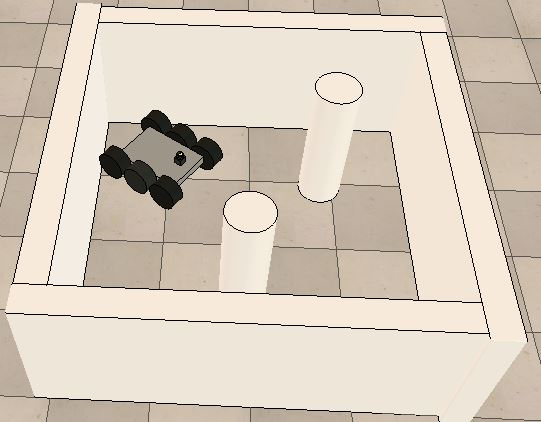
\includegraphics[width=\textwidth]{3d_vrep}
	    \caption{A simulated arena.}
	    \label{fig:3d_vrep}
    \end{subfigure}
    \quad %add desired spacing between images, e. g. ~, \quad, \qquad, \hfill etc.
      %(or a blank line to force the subFigure~onto a new line)
    \begin{subfigure}[b]{0.3\textwidth}
        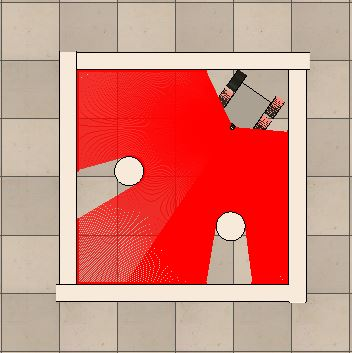
\includegraphics[width=\textwidth]{arena_vrep}
        \caption{Top view.}
        \label{fig:arena_vrep}
    \end{subfigure}%
        \caption{Simulated arena for LIDAR.}
        \label{fig:Simulated_1}
\end{figure}

For the robot to detect the large jumps, the distance is differentiated with respect to angles. As seen in Figure~\ref{fig:Vrep_cylinders}, this will give a specific pattern each time an obstacle (cylindrical in shape) is present. As outlined above,the feature detection may be achieved by considering the derivative of the range data. Namely, each time the derivative is larger than a fixed threshold and is a negative number, n object's beginning is found, and its end is found when a large positive value is encountered. Finding the midpoint of these two readings the location of the cylinder is found as in Figure~\ref{fig:Vrep_cylinders}. 
\begin{figure}
        \centering

        \begin{subfigure}[b]{0.48\textwidth}
                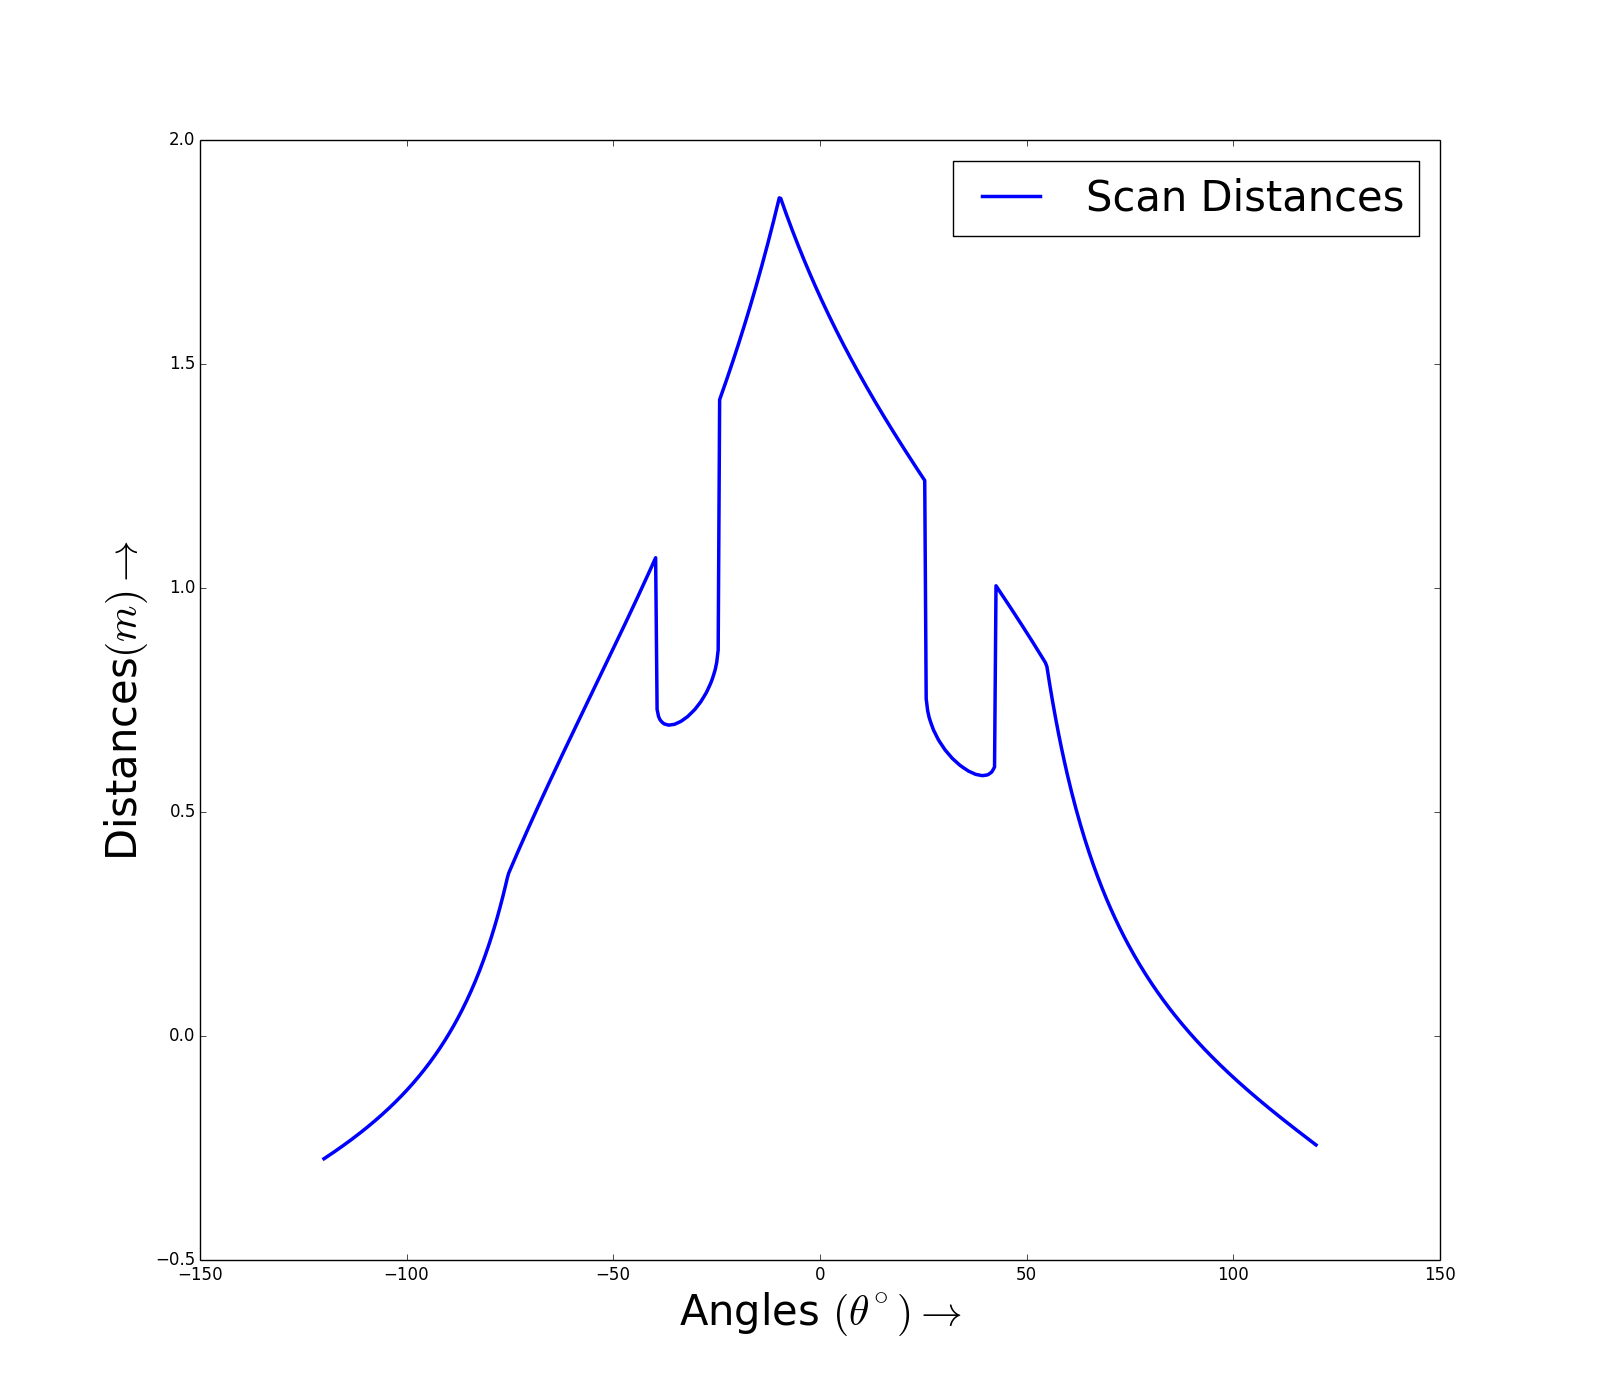
\includegraphics[width=\textwidth]{Vrep_plot}
                \caption{LIDAR scan.}
                \label{fig:Vrep_plot}
        \end{subfigure}
        \quad
        \begin{subfigure}[b]{0.48\textwidth}
                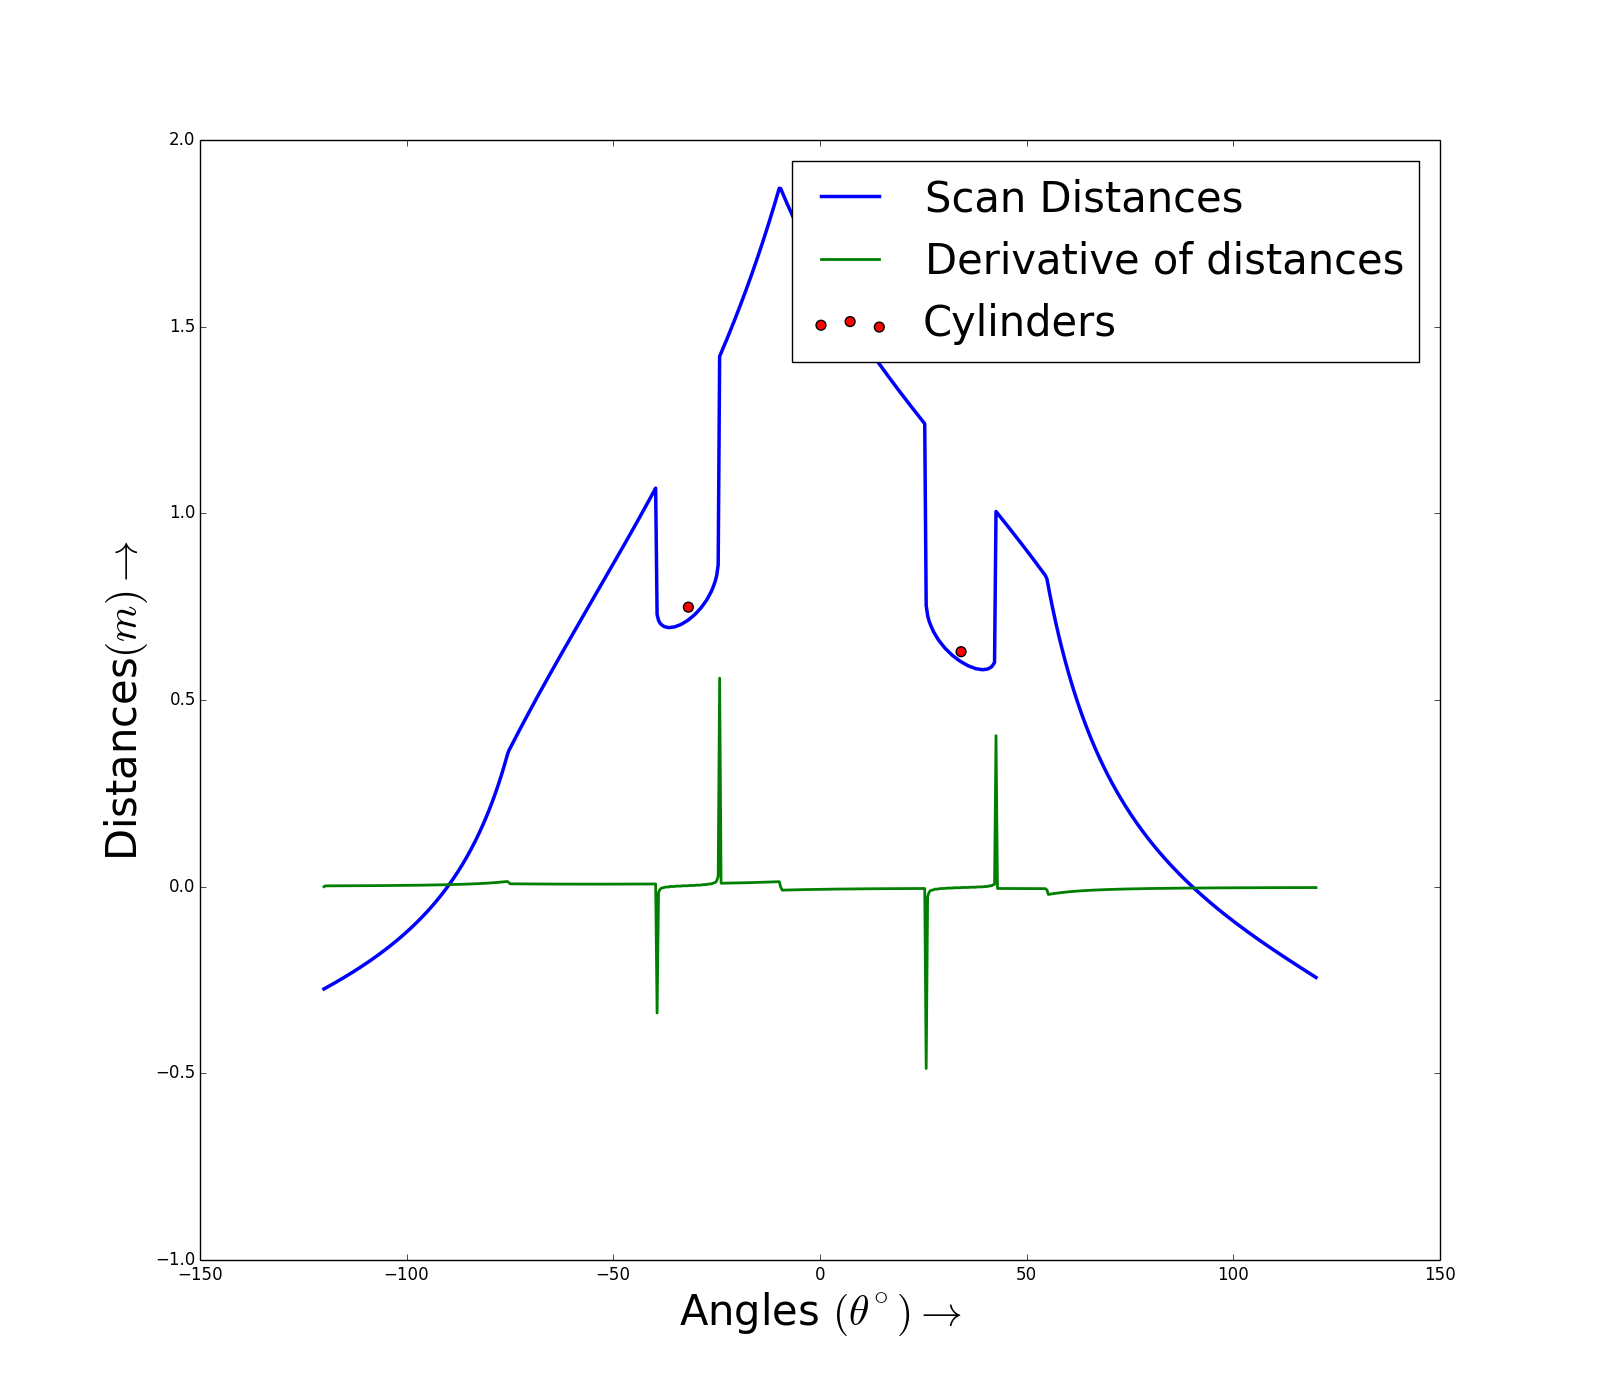
\includegraphics[width=\textwidth]{Vrep_cylinders}
                \caption{Detected cylinders.}
                \label{fig:Vrep_cylinders}
        \end{subfigure}

        \caption{Differential based LIDAR feature detection.}
        \label{fig:Simulated_2}
\end{figure}

It is apparent that this method has a large number of drawbacks. For example, if the arena is larger than the range of the LIDAR. At the points that the distance to any surface is greater than the LIDAR range, a zero value is returned. Leaving these values as zero, will introduce breaks in the range data which will have a detrimental affect on extracting features using the method of differentials outlined above. Another drawback is when there is an obstacle placed very close to a wall. The change in differentials corresponding to the obstacle are much smaller than the change corresponding to other landmarks. Reducing the threshold of differential jump will result in any small features of the arena such as doors being classified as obstacles. Hence it is seen, the choice of threshold for the change in derivative is a very sensitive tuning factor. 

To overcome the above shortcomings, a filter can be designed based on preexisting knowledge of the nature of features. A low threshold is set for the derivative of the range, which results in a large number of obstacles being detected. This set of obstacles is then thinned down by eliminating unlikely detections. Fist filter, is that all obstacles need to have a minimum number of non-zero LIDAR readings that lie on them. Based on the a priori known information, that the obstacle is in the shape of a cylinder with a known approximate radius, the approximate angular width that a prospective obstacle should occupy is predicted. The difference in the width of a candidate obstacle and the predicted width, can be used to remove a few prospective obstacles. There is still a chance of a segment of wall having the same angular width as the predicted width. This will result in spurious landmarks, hence each of the prospective obstacles are compared to the least square fit line for the same points. If the points all fit largely along the line, then it is a segment of the walls and can be removed from the list of possible candidates. By this method, a small amount of robustness is added to a simplistic algorithm of feature detection. The results of such a filter when applied with EKF can be seen in Section~\ref{sec:Spike_results}.

Once the features are detected, the measurement model from the robot to these features need to be calculated to be used in \ekf SLAM.

%
%
%
%
%
%The arena has to be fully within the range of the sensor, if not there will be breaks in the distance curve that will generate spurious landmarks. This drawback can be easily overcome by creating a zero order hold for those regions. Also any disturbances in the boundaries will also generate spurious landmarks. The threshold for the derivative is a very sensitive tuning parameter. If it is set too high there is an increased chance of missing landmarks placed close to walls and if it is set low, there are a large number of spurious landmarks. 
%
%To overcome this, based on preexisting knowledge of the nature of features a filter can be designed. A low threshold is chosen and a large number of prospective features are enumerated. All those that lack a minimum number of points on them are immediately eliminated. Next, based on the fact that the radius of the cylinders that are the landmarks is known, the angular width of any feature detected can be approximated. From the large set, only the ones within a range around this approximate angular width are retained. Then, the least squares fit is computed to check if the features are indeed cylinders or segments of the wall. Only the features having a large enough curvature are retained. 

\subsection{Examples and Validation on IMP}
\label{sec:Spike_results}

In a clean simulated arena, the efficacy of the first approach are seen in Section~\ref{sec: spikeAlgo}. But in a real world environment, a large number of variations will occur. To demonstrate this a relatively clean real world environment is considered as shown in Figure~\ref{fig:Real world arena}. 
\begin{figure}[h!]
    \centering
    \begin{subfigure}[b]{0.45\textwidth}
    
	    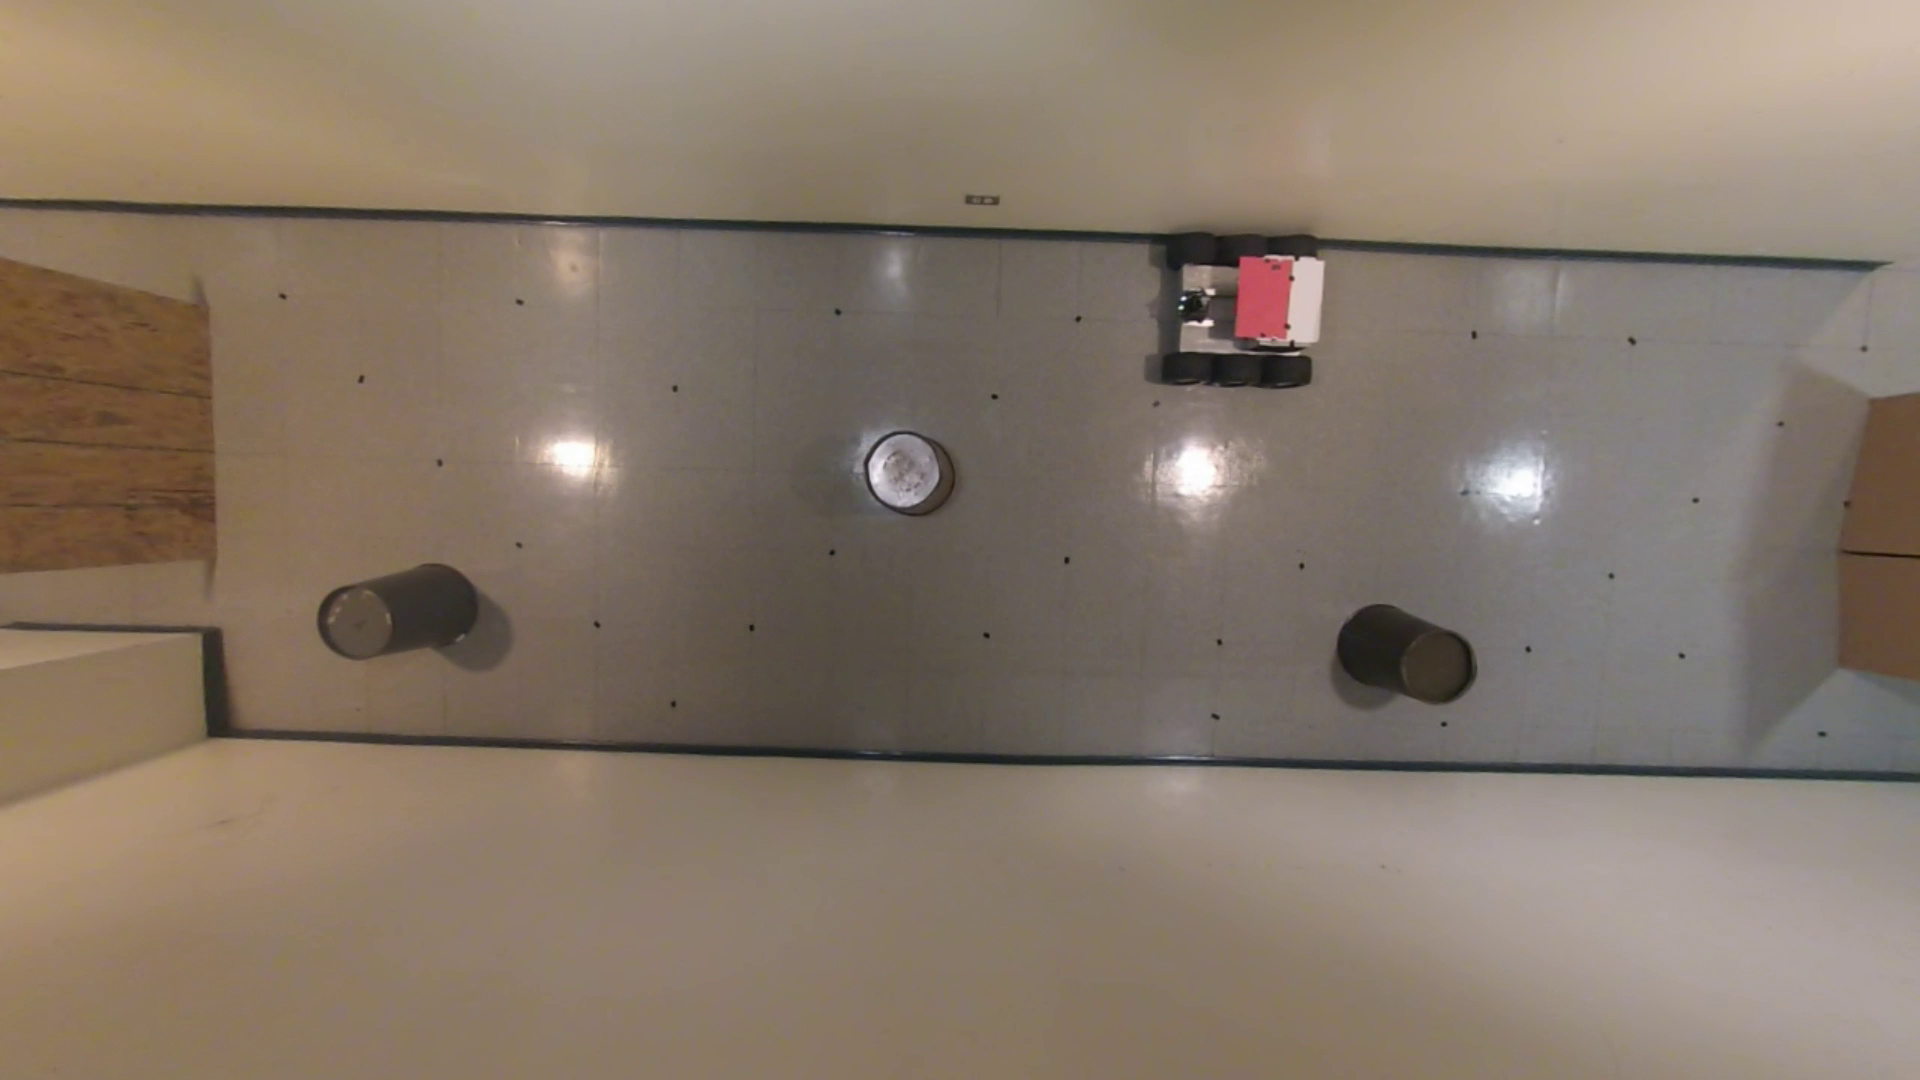
\includegraphics[width=\textwidth]{overhead}
	    \caption{Overhead view.}
	    \label{fig:overhead}
    \end{subfigure}
    \quad %add desired spacing between images, e. g. ~, \quad, \qquad, \hfill etc.
      %(or a blank line to force the subFigure~onto a new line)
    \begin{subfigure}[b]{0.45\textwidth}
        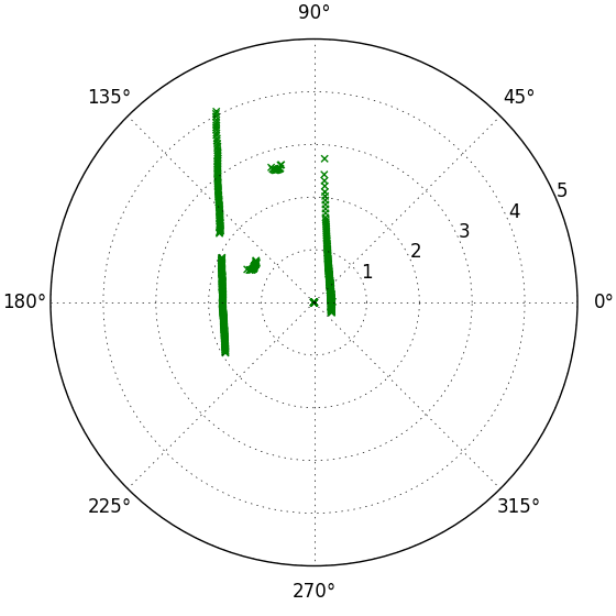
\includegraphics[width=\textwidth]{blank_scan}
        \caption{Polar plot of laser scan.}
        \label{fig:spike_scan}
    \end{subfigure}%
        \caption{Real world arena.}
        \label{fig:Real world arena}
\end{figure}

With such an arena, the simplistic approach of changes in derivatives being obstacles is tried with multiple threshold values.Even in the best case, out of the two obstacles within the range of the LIDAR, only one obstacle gets identified correctly. The other three obstacles detected are incorrect as seen in Figure~\ref{fig:Spike_cylinders_bad}.  

\begin{figure}[h!]
    \centering
    \begin{subfigure}[b]{0.45\textwidth}
	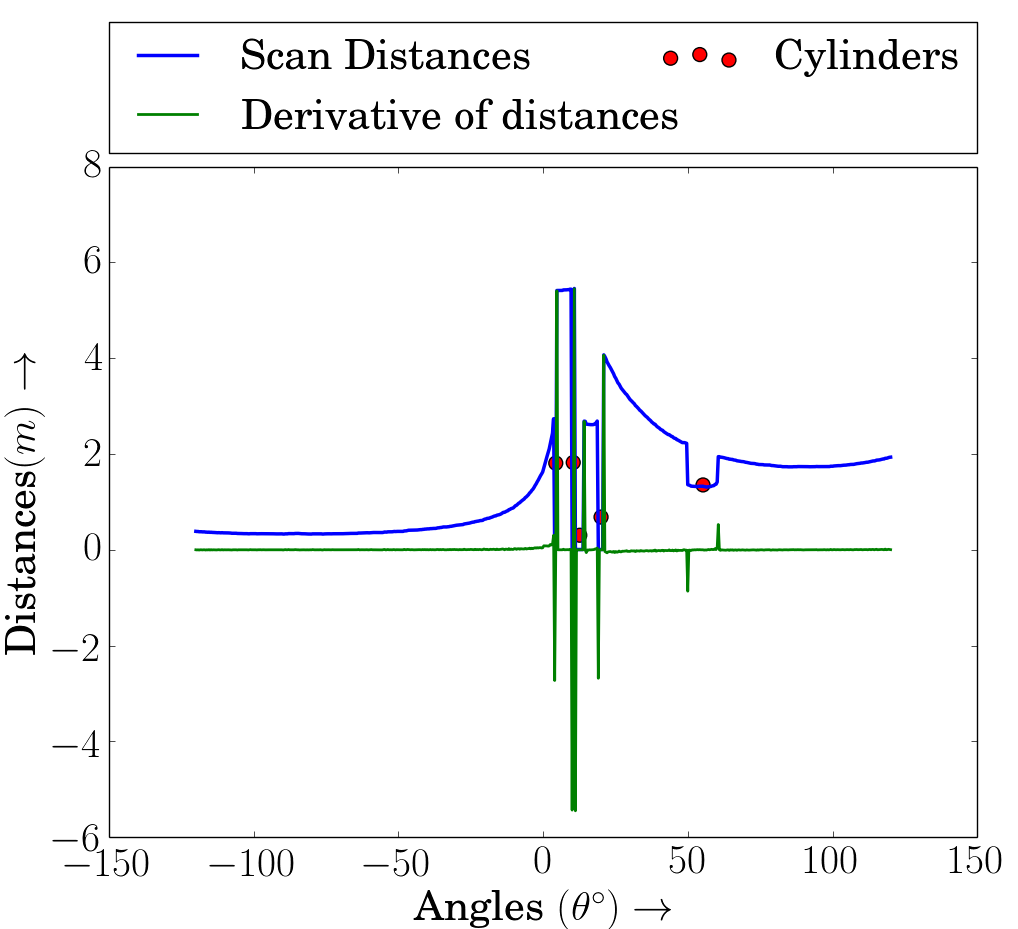
\includegraphics[width=\textwidth]{spike_cyl_bad}
    \end{subfigure}
    \quad %add desired spacing between images, e. g. ~, \quad, \qquad, \hfill etc.
      %(or a blank line to force the subFigure~onto a new line)
    \begin{subfigure}[b]{0.45\textwidth}
        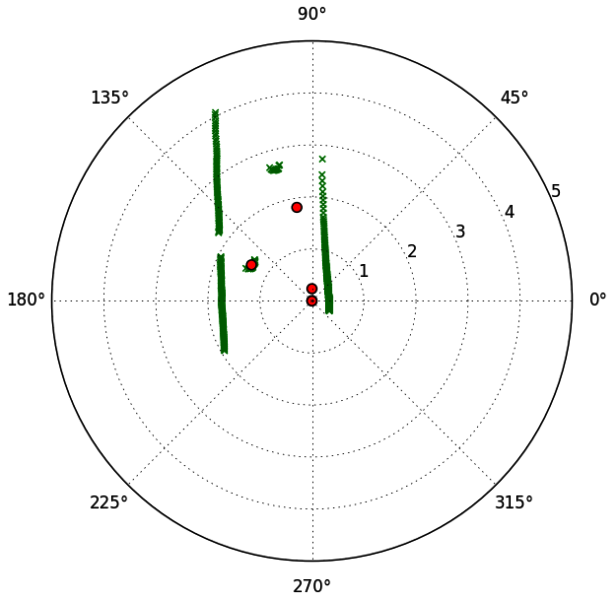
\includegraphics[width=\textwidth]{spike_cyl_badPol}
    \end{subfigure}%
	\caption{Spurious cylinders detected in data.}
	\label{fig:Spike_cylinders_bad}
\end{figure}

\begin{figure}[h!]
\centering
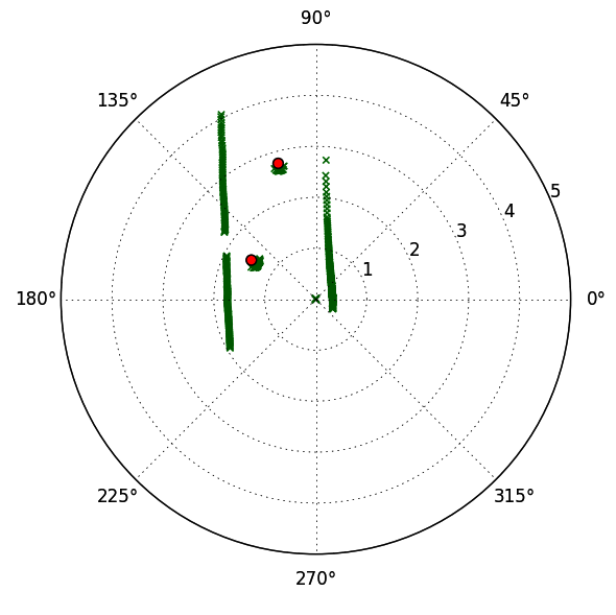
\includegraphics[width=0.4\textwidth]{spike_good}
\caption{After filtering of candidate cylinders.}
\label{fig:spike_good}
\end{figure}

To refine this, conditions similar to those discussed in section \ref{sec: spikeAlgo} are implemented. This is seen to give much better results. as seen in Figure~\ref{fig:spike_good}. 



\subsection{Measurement Model and the Corresponding Jacobian Matrices}
\label{sec:Spike_math}

Once an object's coordinates are found in the LIDAR data, its position has to be stored in the map.  Since an estimate of the robot's position in the inertial frame is known, the object coordinates are mapped from robot to inertial frame using a homogeneous transformation in 2 dimensions as shown in Equation~\ref{eq:SpikeMath1}:
\begin{equation}
\begin{bmatrix}
x_w\\y_w\\1
\end{bmatrix}=
\begin{bmatrix}
\cos(\theta_r) & -\sin(\theta_r) & x_r\\
\cos(\theta_r) & \sin(\theta_r) & y_r\\
0 & 0 & 1
\end{bmatrix}
\begin{bmatrix}
x_1\\y_1\\1
\end{bmatrix}
\label{eq:SpikeMath1}
\end{equation}
where, $ (x_w,y_w) $ are coordinates in the world frame,while $ (x_r,y_r,\theta_r) $ are the estimated pose of the robot and $ (x_1,y_1) $ are the object coordinates in the LIDAR frame.

For, data association, i.e.\ to check if the detected object is being seen for the first time or is being reobserved, the Euclidean distance is used. The euclidean distance between the detected object and the existing object positions is measured and if it is less than a particular threshold then the new object is associated with the existing one. 

For the correction of the robot pose as explained in section \ref{sec:EKF_SLAM}, the measurement model of the point features is needed. This is a mapping that gives the laser reading (i.e.\ range $ r $ and bearing $ \alpha $) from the robot to the object given by Equation \ref{eq:SpikeMath2}:
\begin{equation}
	\label{eq:SpikeMath2}
	h=\begin{bmatrix}
	r\\\alpha
	\end{bmatrix}=
	\begin{bmatrix}
	\sqrt{(y_1-y_r)^2+(x_1-x_r)^2} \\
	\tan^{-1}\left(\frac{y_1-y_r}{x_1-x_r}\right)-\theta_r.
	\end{bmatrix}
\end{equation} 

Using Equation \ref{eq:SpikeMath2} for both the existing landmarks and detected landmarks which have been expressed in the inertial frame, the \textit{innovation} from  Equation~\ref{eq:EKF_8} can be calculated. 

%
%
% the coordinates of the point feature in the robot's frame of reference are found using the inverse of the homogeneous transformation in Equation~\ref{eq:SpikeMath1}. But the robot pose used now is the new position at this particular time step. Once $ (x_1,y_1) $ is found in the robot frame, the measurement h can be found using Equation~\ref{eq:SpikeMath2}. The same equations are used for every corresponding feature that is detected to give $ z $ which is used to calculate the \textit{innovation} in Equation~\ref{eq:EKF_8}.


For the Kalman gain, according to Equation~\ref{eq:EKF_7} the derivatives of the model with respect to the state vector $ x \in \Re^n $ are used. The state contains both the robot pose and all the landmarks already existing in the map at that particular time step. Since it is assumed each landmark is independent of the other, most part of the Jacobian $ H $ contains zeros except for the part corresponding to the robot pose; if the measurement has been associated with an existing landmark, then it will also depend on that landmark's position. Hence for the Jacobian $ H $, the measurement model $ h $ is differentiated as follows:

\begin{equation}
\label{eq:SpikeMath3}
	H = 
	\begin{bmatrix}
	\frac{\partial r}{\partial x_r} & \frac{\partial r}{\partial y_r} & \frac{\partial r}{\partial \theta_r} & \cdots & \frac{\partial r}{\partial x_1} & \frac{\partial r}{\partial y_1} & \cdots \\
	\frac{\partial \alpha}{\partial x_r} & \frac{\partial \alpha}{\partial y_r} & \frac{\partial \alpha}{\partial \theta_r} & \cdots & \frac{\partial \alpha}{\partial x_1} & \frac{\partial \alpha}{\partial y_1} & \cdots 
	\end{bmatrix}.
\end{equation}

Each of the terms in H are derived separately as:


    \begin{equation}
	\frac{\partial r}{\partial x_r} = \frac{(x_r-x_1)}{\sqrt{(y_1-y_r)^2+(x_1-x_r)^2}} \qquad
	\frac{\partial \alpha}{\partial x_r} =  
	\frac{(y_1-y_r)}{(y_1-y_r)^2+(x_1-x_r)^2}
    \end{equation}
	\begin{equation}
    \frac{\partial r}{\partial y_r} = \frac{(y_r-y_1)}{\sqrt{(y_1-y_r)^2+(x_1-x_r)^2}} \qquad
	\frac{\partial \alpha}{\partial y_r} =  
	\frac{(y_r-y_1)}{(y_1-y_r)^2+(x_1-x_r)^2} 
    \end{equation}
	\begin{equation}
    \frac{\partial r}{\partial \theta_r} = 0 \qquad  
	\frac{\partial \alpha}{\partial \theta_r} = -1
    \end{equation}
	\begin{equation}
    \frac{\partial r}{\partial x_1} = \frac{(x_r-x_1)}{\sqrt{(y_1-y_r)^2+(x_1-x_r)^2}} \qquad
	\frac{\partial \alpha}{\partial y_1} =  
	\frac{(y_1-y_r)}{(y_1-y_r)^2+(x_1-x_r)^2} 
    \end{equation}
	\begin{equation}
    \frac{\partial r}{\partial x_1} = \frac{(y_r-y_1)}{\sqrt{(y_1-y_r)^2+(x_1-x_r)^2}} \qquad
	\frac{\partial \alpha}{\partial y_1} =  
	\frac{(y_r-y_1)}{(y_1-y_r)^2+(x_1-x_r)^2}.
    \end{equation}

The only other information needed for Kalman gain calculation is the observer error $ V^TRV $ with V being the derivative of the measurement model with respect to noise. If all landmarks are assumed to be uniformly affected by noise, it is reasonable to approximate V to be an identity matrix. R, the covariance of measurement noise, is a diagonal matrix with one of the eigenvalues representing the error in distance measurement of the LIDAR and the other eigenvalue being the angle measurement.R is given by,
\begin{equation}
\label{eq:SpikeMath5}
R = 
\begin{bmatrix}
\sigma_r & 0 \\
0 & \sigma_\alpha
\end{bmatrix}.
\end{equation}

Using all the measurement model and Jacobian matrices, it is possible to correct the estimate of the robot pose while simultaneously correcting the position of the landmarks. The result of such a \slam  is seen in Section~\ref{cha:results}.
\section{Feature Extraction with Linear Features}
\label{sec:extraction}
\subsection{Overview}
One of the most ubiquitous features of any indoor environment are walls. While it may be necessary to find other obstacles and landmarks for path planning and mapping, knowing the locations of walls tends to be advantageous. At the very least, it can be used to remove all the laser readings that are close to a wall, therefore, reducing the data set to be further analyzed by methods such as clustering. In relatively clean environments such as corridors that are not too crowded, walls will usually suffice for \slam. Also, algorithms that find linear features are more robust to humans moving around in the environment than those finding cylinders or generic features in the data. Also since the feature of interest is a wall, it is reasonable to model it as a line of infinite length which reduces the dimensions of state required to represent it. Similar to Section~\ref{sec:Spike_math}, once the walls have been detected, a measurement model is required to calculate the innovation. It is obvious that the measurement model and its derivatives will not be the same as in point features, as the apparent relative motion of a wall as the robot moves is very different than for point features. For example, when the robot is moving parallel to the wall, the LIDAR scans from one time step to another will be identical, but unlike in the case of point features the similarity of LIDAR scans over successive time steps does not imply that the robot has not moved.

\subsection{RANSAC Based Feature Extraction Algorithm}
\label{sec:ransac}
The fundamental concept in extracting linear features is to fit a line or multiple lines onto a set of points. There are a large number of methods to do this such as least squares, Split-merge and RANSAC\cite{Nguyen2005}. The typical RANSAC-based line extraction in libraries such as OPENCV and PCL, attempt to robustly fit a line to a given set of points. In typical environments, since more than one wall can be seen at a time, it becomes necessary to first segment the data before using the algorithm for demo. Instead, another approach is to randomly sample points and try to fit multiple lines simultaneously.RANSAC finds these line landmarks by randomly taking a sample of the laser readings and then using a least squares approximation to find the best fit line that runs  through these readings. Once this is done RANSAC checks how many laser readings  lie close to this best fit line. If the number is above some threshold we can safely  assume that we have seen a line (and thus seen a wall segment). This threshold is  called the consensus. This approach is explained in algorithm~\ref{alg: RANSAC algorithm}\cite{riisgaard2003slam}. 

\begin{algorithm}[H]
\begin{algorithmic}

	\While{
	\begin{itemize}
		\item there are still unassociated laser readings, 
		\item and the number of readings is larger than the consensus, 
		\item and less than N trials have been done,
	\end{itemize}
	}
	\begin{itemize}
	\item Select a random laser data reading. 
	\item Randomly sample S data readings within D degrees of this laser 
	data reading 
	\item Using these S samples and the original reading calculate a 
	least squares best fit line $ L $. 
	\item Determine how many laser data readings lie within X distance 
	from this best fit line
	\item If the number of laser data readings on the line is above some 
	consensus C do the following: 
		\begin{itemize}
			\item calculate new least squares best fit line based on all 
			the laser readings determined to lie close to the old best fit 
			line. 
			\item Add this best fit line to the lines that have been extracted. 
			\item Remove the number of readings lying close to the line from the 
			total set of unassociated readings.
		\end{itemize}
	\end{itemize}
	\EndWhile
\end{algorithmic}
	\caption{Multiple line fitting with RANSAC.}
	\label{alg: RANSAC algorithm}
\end{algorithm}
This algorithm can thus be tuned based on the following parameters: 
\begin{itemize}
\item N – Max number of times to attempt to find lines. 
\item S – Number of samples to compute initial line. 
\item D – Degrees from initial reading to sample from. 
\item X – Max distance a reading may be from line to get associated to line. 
\item C – Number of points that must lie on a line for itto be taken as a line
\end{itemize}


\subsection{RANSAC Examples}
 \begin{figure}[h!]
     \centering
     \begin{subfigure}[b]{0.45\textwidth}
     
 	    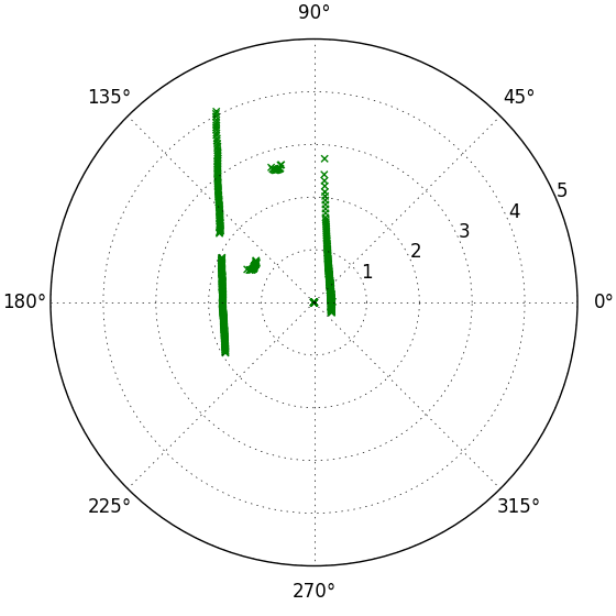
\includegraphics[width=\textwidth]{blank_scan}
         \caption{Polar plot of laser scan.}
     \end{subfigure}
     \quad %add desired spacing between images, e. g. ~, \quad, \qquad, \hfill etc.
       %(or a blank line to force the subFigure~onto a new line)
     \begin{subfigure}[b]{0.45\textwidth}
         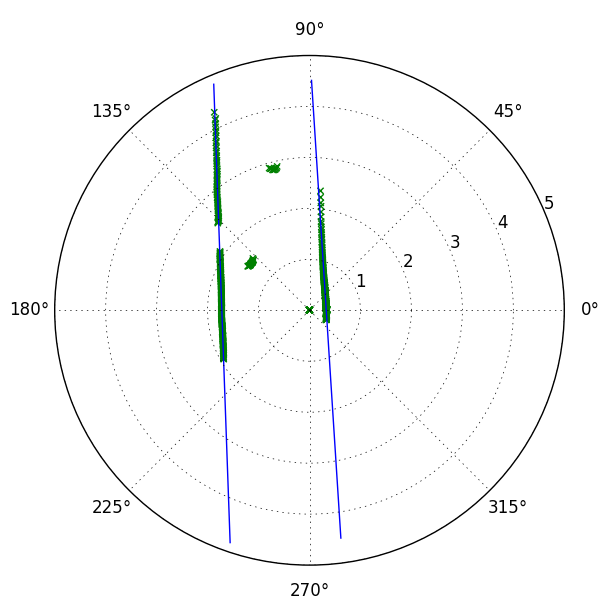
\includegraphics[width=\textwidth]{ransac_good}
		 \caption{Detected lines.}
     \end{subfigure}%
         \caption{Example of walls detected by RANSAC.}
         \label{fig: ransac_good}
 \end{figure}
 Considering the same setup as in Figure~\ref{fig:Real world arena}, we can try the RANSAC algorithm on the data collected from the LIDAR. It is initially seen to give good results as seen in Figure~\ref{fig: ransac_good}. However, the robustness of the algorithm is not consistant. As we move forward though, the robustnes is not always maintained. Looking at algorithm~\ref{alg: RANSAC algorithm} it is possible that since the first laser reading is chosen at random, it may not be on a wall at all. S readings in its neighborhood could generate a line that is at a small angle to both walls in the environment. Since it is close enough to the walls, a large number of points will wrongly be associated to this, which will result in a spurious wall being detected.This will have a detrimental effect in all the further time steps. An example of this is seen in Figure~\ref{fig: ransac_bad}.
 \begin{figure}[h!]
     \centering
     \begin{subfigure}[b]{0.45\textwidth}
     
 	    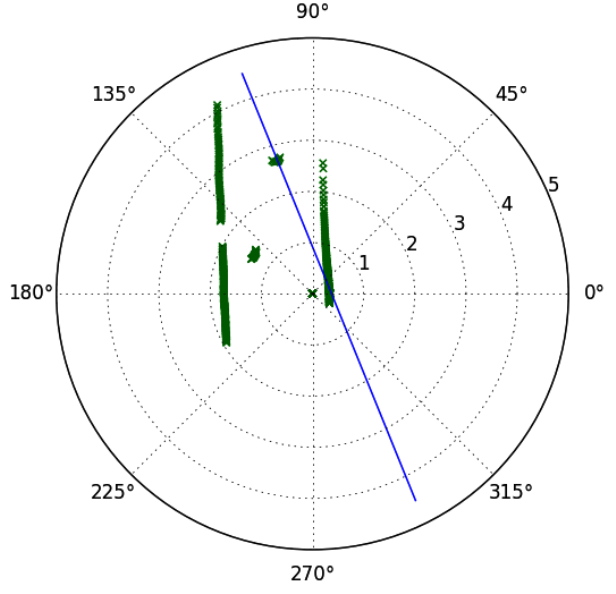
\includegraphics[width=\textwidth]{ransac_bad}
        \caption{Detected lines.}
     \end{subfigure}
     \quad %add desired spacing between images, e. g. ~, \quad, \qquad, \hfill etc.
       %(or a blank line to force the subFigure~onto a new line)
     \begin{subfigure}[b]{0.45\textwidth}
         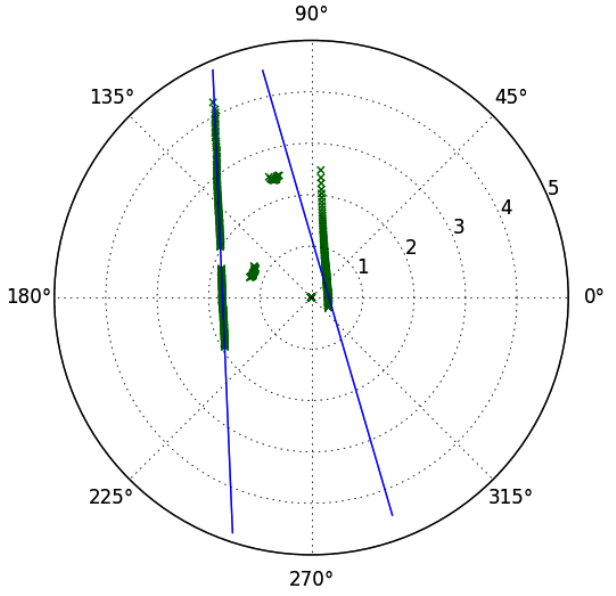
\includegraphics[width=\textwidth]{ransac_bad1}
		 \caption{Detected lines.}
     \end{subfigure}%
         \caption{Example of spurious walls marked by RANSAC.}
         \label{fig: ransac_bad}
 \end{figure}
\subsection{Hough Transform Based Feature Extraction Algorithm}
\label{sec:hough}
In the fields of image analysis and computer vision, the Hough transform is a very popular feature extraction technique\cite{Stockman2001}. While it was originally designed to find lines in an image, it can also be used to detect any shape as long as that shape can be represented in a parametric form\cite{Duda1972}. This algorithm can detect a shape in spite of distortions making it much more robust than the RANSAC based algorithm shown in Algorithm~\ref{alg: RANSAC algorithm}\cite{Hu1998}. In the current application, the aim is to find walls in the range data of the LIDAR. Hence, the first step is to rasterize the points into an image so that we can use the OpenCV implementation of Hough transform. The image is then converted to a binary image and passed to the Hough transform function. The algorithm itself is described below.

In image processing, a common way of representing lines is the normal form of a line equation, 
\begin{equation}
r=x\cos\theta+y\sin\theta.
\label{eq:hough1}
\end{equation}
In this form a line is completely defined by 2 variables $ r $ and  $ \theta $. Note that for any point $ (x_0,y_0) $ in the image, a family of lines passing through that point is expressed as,

\begin{equation}
r_\theta=x_0\cos\theta+y_0\sin\theta.
\label{eq:hough2}
\end{equation}

Since all lines are assumed to be infinite in both directions, $ \theta $ can only take unique values between $ 0^\circ $ and $ 180^\circ $. This range is then discretized to give a fixed number of possible line angles. The range $ r $ is also discretized based on the resolution required. For single pixel resolution, the possible ranges will be all numbers from 0 to the length of the diagonal of the image. Since this will result in a large number of possible $ r $ values, a lower resolution will considerably speed up the algorithm. Now that there is a fixed number for possible $ r $ and $ \theta $, a 2D matrix of zeros is created in which each row corresponds to a possible value of $ \theta $ and each column to $ r $ as in Equation~\ref{eq:hough3}. This is called the accumulator:

\begin{equation}
A=\bordermatrix{~  & r_1 & r_2&\ldots & r_n \cr
              \theta_1& 0 &  0  & \ldots & 0\cr
              \theta_2& 0  &  0 & \ldots & \cr
              \vdots& \vdots & \vdots & \ddots & \vdots\cr
              \theta_n& 0  &   0       &\ldots & 0}.
\label{eq:hough3}
\end{equation} 

 Once this initial setup is complete, a non zero point on the binary image $ (x_0,y_0) $ is chosen at random. For this point, the family of lines passing through it will be given by Equation~\ref{eq:hough2}. For each possible $ \theta $ the corresponding $ r $ is calculated from the same equation. For each $ (r,\theta) $ pair found, the corresponding entry in the accumulator $ A $ is incremented. Once all the possible pairs are calculated, a different image point is chosen till all the non zero points on the image are explored. 
 
 The accumulator now represents all possible lines in the image and the number of points that lie on each of the lines. The accumulator entries that are greater than a threshold represent the lines in the image. The $ (r,\theta) $ values corresponding to these lines are returned. 
 
 An important aspect of using the ransform from OpenCV is the conversion of LIDAR data to an image and the detected lines back to the robot frame of reference. The former is straightforward. Since the range of the LIDAR is known, the image size can be fixed based on the resolution required. For, example the LIDAR described in Chapter~\ref{cha:Platform } has a maximum range of 5 m. So for a resolution of 1 cm, a blank image of $ 500 \times 500 $ pixels is created. When each LIDAR point is converted to Cartesian coordinates $ (x_l,y_l) $, they are with respect to an origin at the LIDAR itself. OpenCV images on the other hand follow a coordinate system that has the origin in the top right corner of the image. Hence, each point is mapped to the image coordinate frame using a homogeneous transformation given as
 \begin{equation}
 \begin{bmatrix}
 x_i\\y_i\\1
 \end{bmatrix}=
 \begin{bmatrix}
 0 & -1 & 500\\
 1 & 0 & 500\\
 0 & 0 & 1
 \end{bmatrix}
 \begin{bmatrix}
 x_l\\y_l\\1
 \end{bmatrix}.
 \label{eq:hough4}
 \end{equation}
 
The image points are then rounded to the nearest centimeter and the pixel corresponding to that value is set to white. This gives an image with black background and all the Laser readings shown in white which can be passed to the Hough transform function.

% It may sometimes be required to erode and dilate the image with different kernels to make the points more visible. 
 
The lines returned by the Hough transform, are in units of pixels and are with reference the image origin. To convert it to the robot frame, 2 points are chosen on the line and each of these points are mapped to the robot frame using the inverse transformation of Equation~\ref{eq:hough4} and the normal form of the equation of a line passing through these 2 points is found. 

\subsection{Hough Transform Examples}
In the same arena as in Figure~\ref{fig:Real world arena}, the Hough transform is found to be really robust in finding the walls as seen in Figure~\ref{fig: hough1}.
 \begin{figure}[h!]
     \centering
     \begin{subfigure}[b]{0.45\textwidth}
     
 	    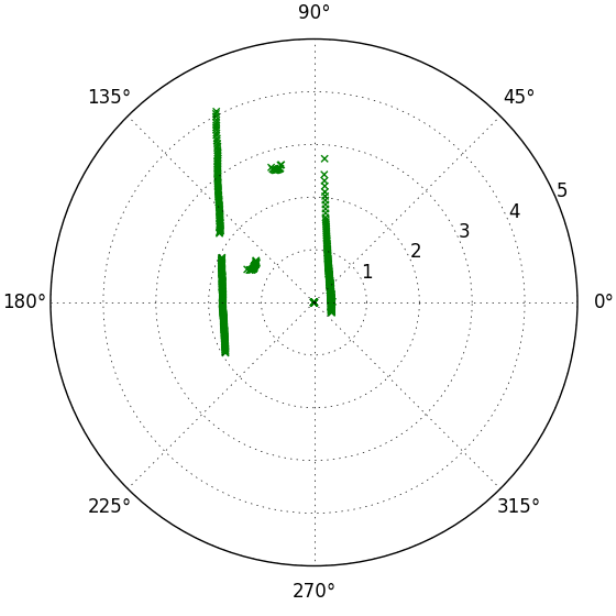
\includegraphics[width=\textwidth]{blank_scan}
         \caption{Polar plot of laser scan.}
     \end{subfigure}
     \quad %add desired spacing between images, e. g. ~, \quad, \qquad, \hfill etc.
       %(or a blank line to force the subFigure~onto a new line)
     \begin{subfigure}[b]{0.45\textwidth}
         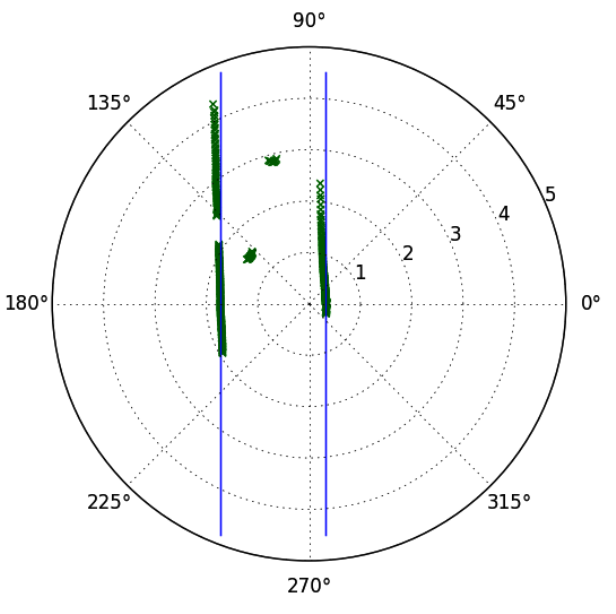
\includegraphics[width=\textwidth]{hough1}
		 \caption{Detected lines.}
     \end{subfigure}%
         \caption{Example of walls detected by Hough transform.}
         \label{fig: hough1}
 \end{figure}

Unlike the RANSAC algorithm, the Hough transform considers all possible lines before deciding on any line and is robust to noise in the surroundings. This is especially useful when there are people walking around in the environment.
 \begin{figure}[h!]
     \centering
     \begin{subfigure}[b]{0.45\textwidth}
     
 	    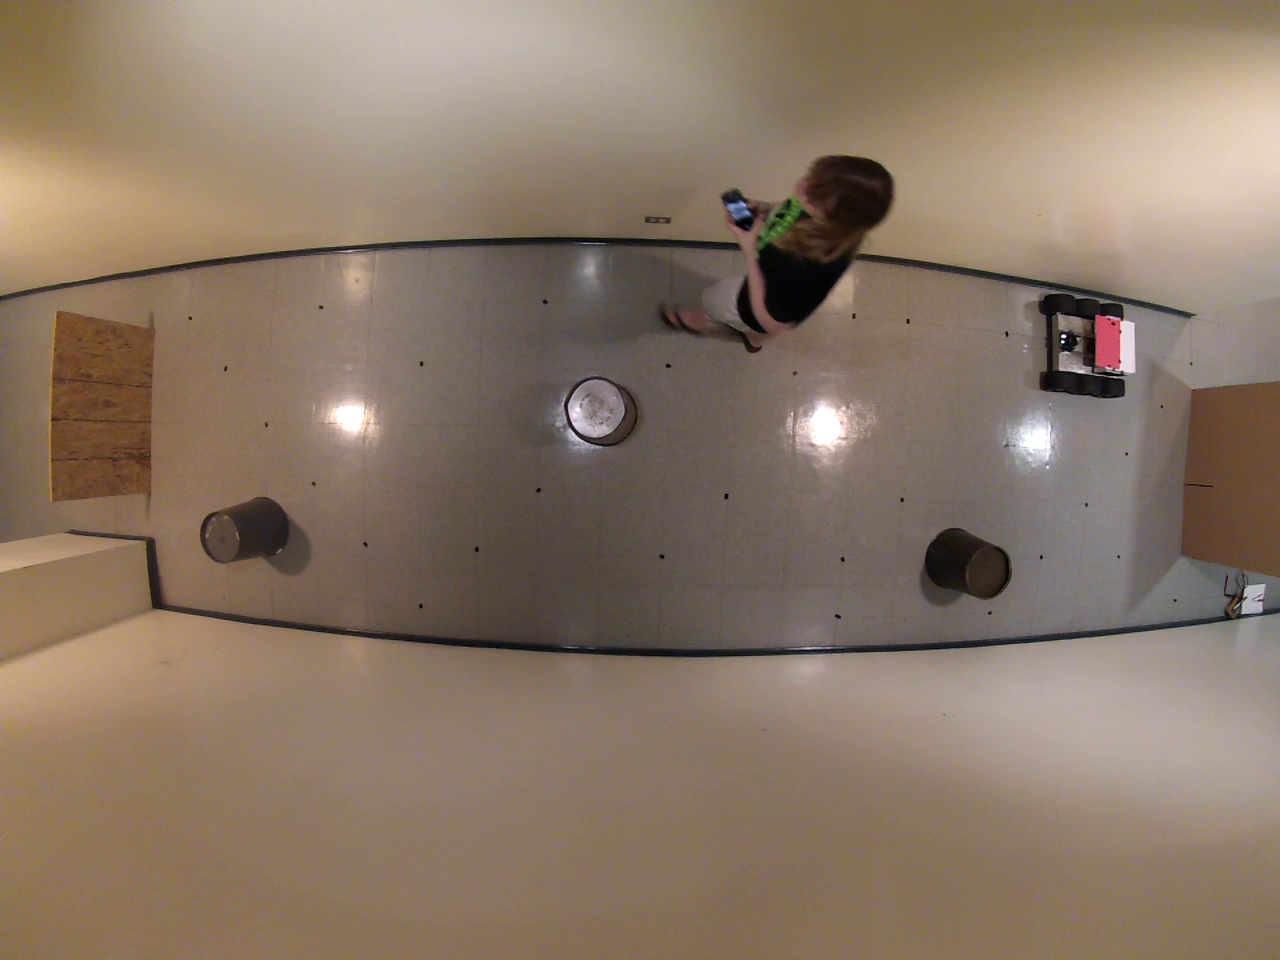
\includegraphics[width=\textwidth]{overhead2}
         \caption{Overhead view of the arena.}
     \end{subfigure}
     \quad %add desired spacing between images, e. g. ~, \quad, \qquad, \hfill etc.
       %(or a blank line to force the subFigure~onto a new line)
     \begin{subfigure}[b]{0.45\textwidth}
         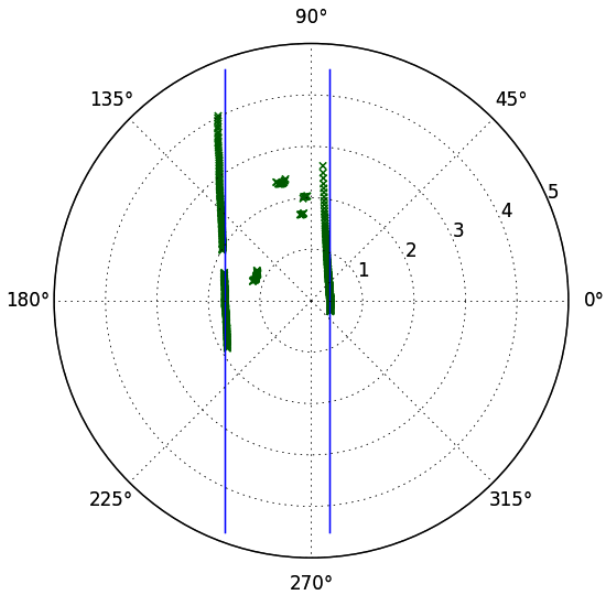
\includegraphics[width=\textwidth]{hough2}
		 \caption{Detected lines}
     \end{subfigure}%
         \caption{Example 1 of Hough transform being robust to additional objects (e.g.,\ people) in the environment.} 
         \label{fig: hough2}
 \end{figure}
 
  \begin{figure}[h!]
      \centering
      \begin{subfigure}[b]{0.45\textwidth}
      
  	    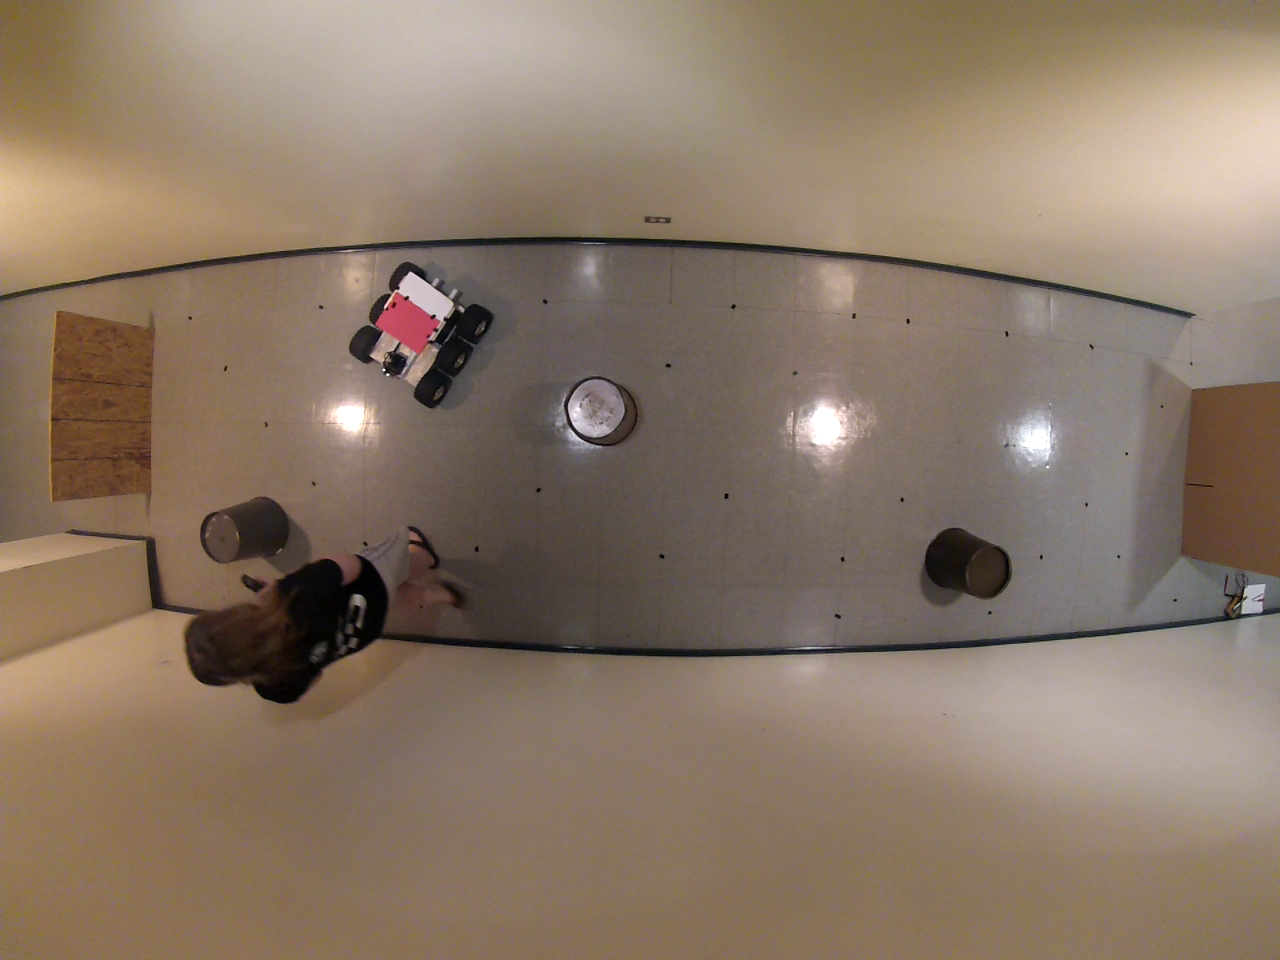
\includegraphics[width=\textwidth]{overhead3}
          \caption{Overhead view of the arena}
      \end{subfigure}
      \quad %add desired spacing between images, e. g. ~, \quad, \qquad, \hfill etc.
        %(or a blank line to force the subFigure~onto a new line)
      \begin{subfigure}[b]{0.45\textwidth}
          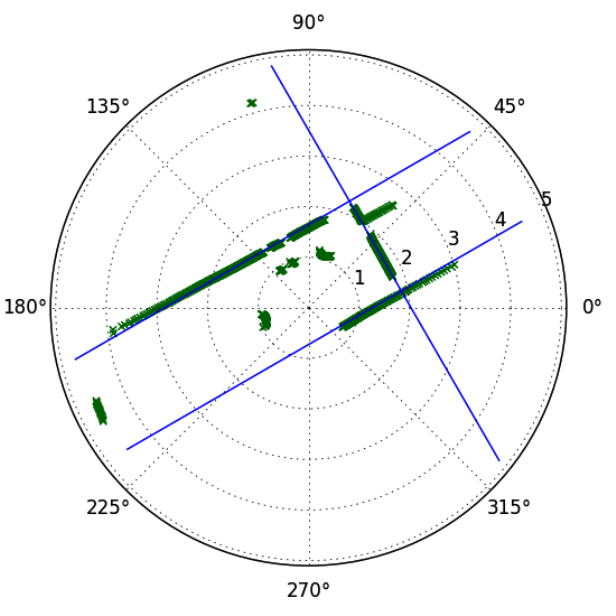
\includegraphics[width=\textwidth]{hough3}
 		 \caption{Detected lines}
      \end{subfigure}%
          \caption{Example 1 of Hough transform being robust to additional objects (e.g.,\ people) in the environment.}
          \label{fig: hough3}
  \end{figure}
 
\subsection{Measurement Model and the Corresponding Differentials}
\label{sec:linear_math}
Once the lines in the data are recovered, the lines need to be expressed in an effective format to store them. The common, slope-point form has a major disadvantage when trying to represent perfectly vertical lines and the two point form will expand the size of the measurement vector $ z $ increasing the calculation required for \ekf. So it is preferable to represent it in the normal form where just the coordinates of the point of intersection of the normal from the origin to the line is stored. For example, in Figure~\ref{fig: normal_form}, the line can be represented solely by the point $ D $.

\begin{figure}
\centering
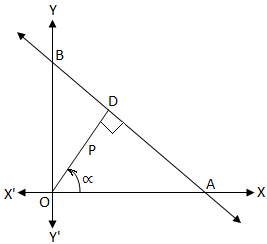
\includegraphics[width=0.45\textwidth]{normal_form_2}
\caption{Normal form of a line.}
\label{fig: normal_form}
\end{figure}

As in Section~\ref{sec:Spike_math}, the line coordinates have to be converted to the inertial frame of reference.For Example, in Figure~\ref{fig: wall_to_world}, the point $ P_1 $ in robot frame is known and point $ P_2 $ has to be found in the inertial frame given coordinates of the robot in inertial frame as $ P_r $(refer Algorithm~\ref{alg: wall_to_world}).
\begin{figure}
\centering
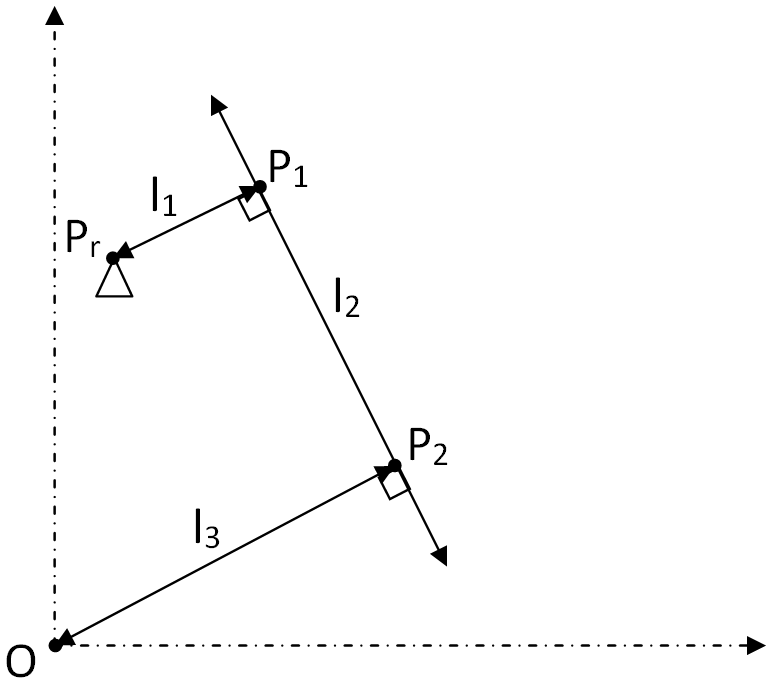
\includegraphics[width=0.45\textwidth]{wall_to_world}
\caption{Line in robot frame and world frame.}
\label{fig: wall_to_world}
\end{figure}

\begin{algorithm}[]
	\begin{enumerate}
		\item Convert point $ P_1 $ from robot frame to inertial frame as in Section~\ref{sec:Spike_math}
		\item Given points $ P_r $ and $ P_1 $ in inertial frame, the equation of line $ l_1 $ can be foundby connecting few points. 
		\item Since $ l1 \perp l2 $, the slope of $ l_2 $ is the negative reciprocal of the slope of $ l_1 $. 
		\item Using the slope and the point $ P_1 $ the Equation~of line $ l_2 $ is found using slope-point form of a line.
		\item The equation~of line l3 is found similarly using slope of $ l_1 $ and point $ O $. 
		\item The coordinates of point $ P_2 $ are obtained by solving equations for $ l_3 $ and $ l_2 $.
	\end{enumerate}
\caption{To convert linear features from robot frame to inertial frame.}
\label{alg: wall_to_world}
\end{algorithm}

Once the landmark is in the world frame,its corresponds to any existing landmark in the map can be checked. This can be checked by comparing both the perpendicular distances between the walls and the angle between the walls. This allows us to have 2 tuning parameters so that the association can be weighted as desired. Usually, since most walls in an indoor environments are at right angles, the variation allowed in angle for the association is larger compared to distance. 

Algorithm~\ref{alg: wall_to_world} is also called the inverse measurement model since in subsequent time steps for the measurement model is obtained by the exact opposite process: That is given a line using its normal form in inertial frame, get the \textit{measurement} from the robot. That is, we need the perpendicular distance from the robot to the wall and the angle of the laser beam which would hit the wall perpendicularly. For this given coordinate pf point $ P_2 $ as $ (x_2,y_2) $ and the robot pose as $ (x_r,y_r,\theta_r) $, the Cartesian coordinates $ P_1 $ is calculated as: % using Equation~\ref{eq:lineModel1}. 

\begin{equation}
	\label{eq:lineModel1}
	x_1 = x_2 - \frac{y_2 ( x_2 y_ r- y_2 x_r)}{(x_2^2 + y_2^2)}
	\qquad
	y_1 = y_2 + \frac{x_2 ( x_2 y_ r- y_2 x_r)}{(x_2^2 + y_2^2)}.
\end{equation}

Once $ P_1 $ is known,the perpendicular distance $ r $ and angle $ \alpha $ are calculated using Equation~\ref{eq:lineModel2}:
\begin{equation}
	\label{eq:lineModel2}
	r=\sqrt{(y_1-y_r)^2+(x_1-x_r)^2}
	\qquad
	\alpha = \tan^{-1}\left(\frac{y_1-y_r}{x_1-x_r}\right)-\theta_r,
\end{equation}
giving measurement model $ h $ as per Equation~\ref{eq:lineModel3}
\begin{equation}
	\label{eq:lineModel3}
	h=\begin{bmatrix}
	r\\\alpha
	\end{bmatrix}.
\end{equation}

For calculating the \textit{Kalman gain}, we need the Jacobian matrix $ H $. As each wall is independent of the other, this has the same structure as explained in Section~\ref{sec:Spike_math} and is given by Equation~\ref{eq:SpikeMath3}. Each of the terms on H is derived individually. The 
 A factor common to all the components of the Jacobian is given by:

  \begin{equation}	
	\beta = \frac{x_rx_1-x_1^2-y_1^2+y_ry_1}{x_1^2+y_1^2}.
  \end{equation}

The part of the Jacobian with respect to the position of the robot is:
  \begin{equation}
	\frac{\partial r}{\partial x_r} = 2x_1\beta \quad
	\frac{\partial r}{\partial y_r} = 2y_1\beta \quad
	\frac{\partial r}{\partial \theta_r} = 0 
  \end{equation}
  \begin{equation}
	\frac{\partial \alpha}{\partial x_r} = 0 \quad 
	\frac{\partial \alpha}{\partial y_r} = 0 \quad 
	\frac{\partial \alpha}{\partial \theta_r} = -1.
  \end{equation}
In these equations, it is seen that, $ \alpha $ is independent of the location of the robot and is inversely proportional to the orientation. Since $ r $ and $ \alpha $ are in the robot frame of reference. For a given wall, as long as the robot is facing the same direction, the angle at which the wall is seen remains the same. Similarly the perpendicular distance $ r $ between a robot center and a wall will remain the same irrespective of the orientation of the robot. 

Differentiating with the obstacle positions gives us the following:
	\begin{equation}
  \frac{\partial r}{\partial x_1} = -2x_1\beta^2 - 2\beta(2x_1-x_r)
  \end{equation}

  \begin{equation}
	\frac{\partial r}{\partial y_1} = -2y_1\beta^2 - 2\beta(2y_1-y_r)
	\end{equation}
  \begin{equation}
  \frac{\partial \alpha}{\partial x_1} =  \frac{-y_1}{x_1^2+y_1^2}\qquad
	\frac{\partial \alpha}{\partial y_1} =
	\frac{x_1}{x_1^2+y_1^2} .
	\end{equation}


Having the Jacobian matrices we can use the same observer error given by Equation~\ref{eq:SpikeMath5} to correct the position estimate using equations~\ref{eq:EKF_7} to~\ref{eq:EKF_9}.





\section{Measurement Model and the corresponding differentials}
\textit{The mathematical model for measurement.}

\section{Experimental results}
\textit{Description of the arena and the run performed.}

\textit{Images of the path ground truth and correction.}

\textit{It gives good estimate of walls and is much faster.}
 
\chapter{Visual odometry}

\section{Overview}

Traditionally a Camera is used as and exteroceptive sensor to get measurements of the environment. But it is interesting how it can also be used as a proprioceptive sensor using visual odometry\cite{}. By this, the number of sensors on a robot can be reduced saving cost and weight which are of extreme importance in certain cases. 


\section{Conceptual Description}
\textit{Description of epipolar geometry}
\textit{The mathematical base for visual odometry}

\section{Implementation and integration with EKF SLAM}
\textit{Visual odometry based motion model and Jacobian}

\section{Experimental results}
\textit{Description of the arena and the run performed.}
\textit{Images of the path ground truth and prediction.}
\textit{Images of the path ground truth and correction.}

Not as good. But good enough. Shown using corrected path
 
%\chapter{Implementation and Results}
\label{cha:results}

\section{Implementation of EKF SLAM algorithm}
\label{sec:slam_process}
The SLAM algorithm, as discussed in chapter \ref{cha:Overview}, consists of subparts each of which present challenges of its own. The primary purpose of this thesis is to develop a flexible implementation that can accommodate different algorithms for the subparts,hence, the guiding principle of the implementation is modularity. Hence an object oriented language such as Python is the platform of choice. This allows us to create individual objects for each part of the algorithm which can be substituted with ease to utilize different combinations of algorithms for feature extraction, association and filtering. 

During the initial setup, all the objects are created and initialized. A robot object is instantiated with its initial position and covariance representing the uncertainty in its position. This object holds the robot's position and uncertainty all through the runtime. It also contains objects for all the sensors and components that the actual robot contains. For example, an object of ENCODER class is instantiated with all its properties such as its noise factors, the diameter of the wheels it is attached on, and the separation between the wheels. A LIDAR object is also instantiated with the minimum and maximum range of the Hokuyo, the offset of the LIDAR from the center of the platform, and the measurement noise factors. These sensor objects are attached to the Robot object into proprioceptive and exteroceptive sensor lists, respectively. The proprioceptive sensors contain methods to calculate the motion model of the robot and also its Jacobian matrices.
To the exteroceptive sensors, feature extractor objects are attached. Each feature extraction algorithm is implemented as its own class. All such classes have to have a particular structure based on the sensor whose data the extractor uses. For LIDAR based extractors,  there has to be a function called \textit{get\_landmarks()} which takes in angles and distances and returns a list of landmark locations. They also need a member variable named \textit{landmarkType} which contains the type of landmark that the extractor is trying to find. 

The exteroceptive sensors are designed to take the list of landmark positions from each feature extractor attached to them and create objects of LANDMARK class for them. A combined list of landmark objects from all the feature extractors is returned by the exteroceptive sensor class. These landmark objects are objects of the LANDMARK class. This is a factory class which, for example, returns objects of either WALL or CYLINDER based on the \textit{landmarkType} returned by \textit{get\_landmarks}. Each of these classes contain methods to calculate their measurement models and their Jacobian matrices.
The main part of SLAM is carried out by an object of EKF class. This object contains  state and covariance members which represent the whole environment. In SLAM along with the robot's position being updated, the environment also needs to be mapped. So a representation of the environment called the map is held by an object of EKF class. It is essentially a list of all robot and landmark objects created.

\begin{figure}
\centering
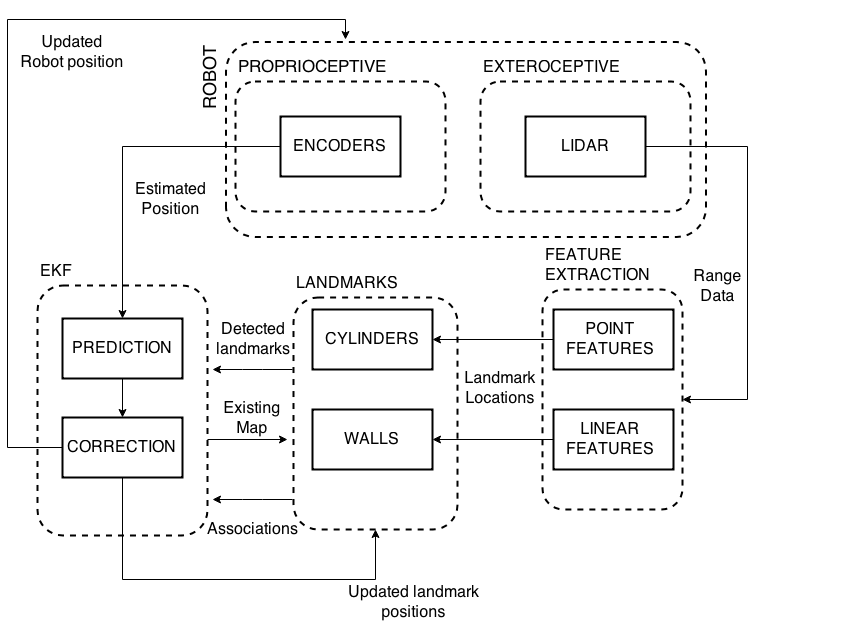
\includegraphics[width=\textwidth]{slam_process}
\caption{SLAM Implementation using only LIDAR}
\label{fig:slam_process}
\end{figure}
Once initial setup is made, the robot object is added to the EKF map. Then for each time step, the \textit{run()} method of the EKF object is called. In this function the first step is prediction wherein for each robot in the map, the \textit{predict()} method of the robot object is called. That in turn calls the \textit{update()} method of all the proprioceptive sensors attached to that robot. This gives the estimated position and uncertainty using equation \ref{eq:Enc_3}. 

Then the \textit{observe()} method of the robot is called which in turn calls the exteroceptive sensors which generate landmark objects for all the landmarks seen at that time step. Each of these landmark objects are then checked to see if they are associated with a landmark preexisting in the map. For each re-observed landmark, the innovation and Kalman gain are calculated and the whole state is corrected. The map objects are then updated with the corrected positions. 

\section{Experimental Results}

To test the impact of the two feature extraction algorithms discussed in Chapter~\ref{cha:featureExtractors} on \slam, the \imp was driven around in first a controlled and then an uncontrolled indoor environment while continuously logging data. The Encoder and IMU data was logged at high speed at 100 Hz, and the LIDAR and Camera was logged at 5 Hz. The logged data was then analyzed using an EKF SLAM algorithm implemented as described in Section~\ref{sec:slam_process}. 

In the controlled environment, the two ends of a regular corridor are sealed off resulting in a closed space with no other features except walls and cylinders placed intentionally. This enables us to test the point feature extraction algorithm and see its effect on SLAM both individually and in combination with Hough transform based linear feature extraction. The controlled environment along with the path taken by IMP is seen in Figure~\ref{fig:overhead_path}. The closed-off space is still large enough such that it is not entirely within the range of the LIDAR. Hence, the problems and modifications discussed in Chapter~\ref{cha:featureExtractors} are still relevant even in a clean environment. 
\begin{figure}
\centering
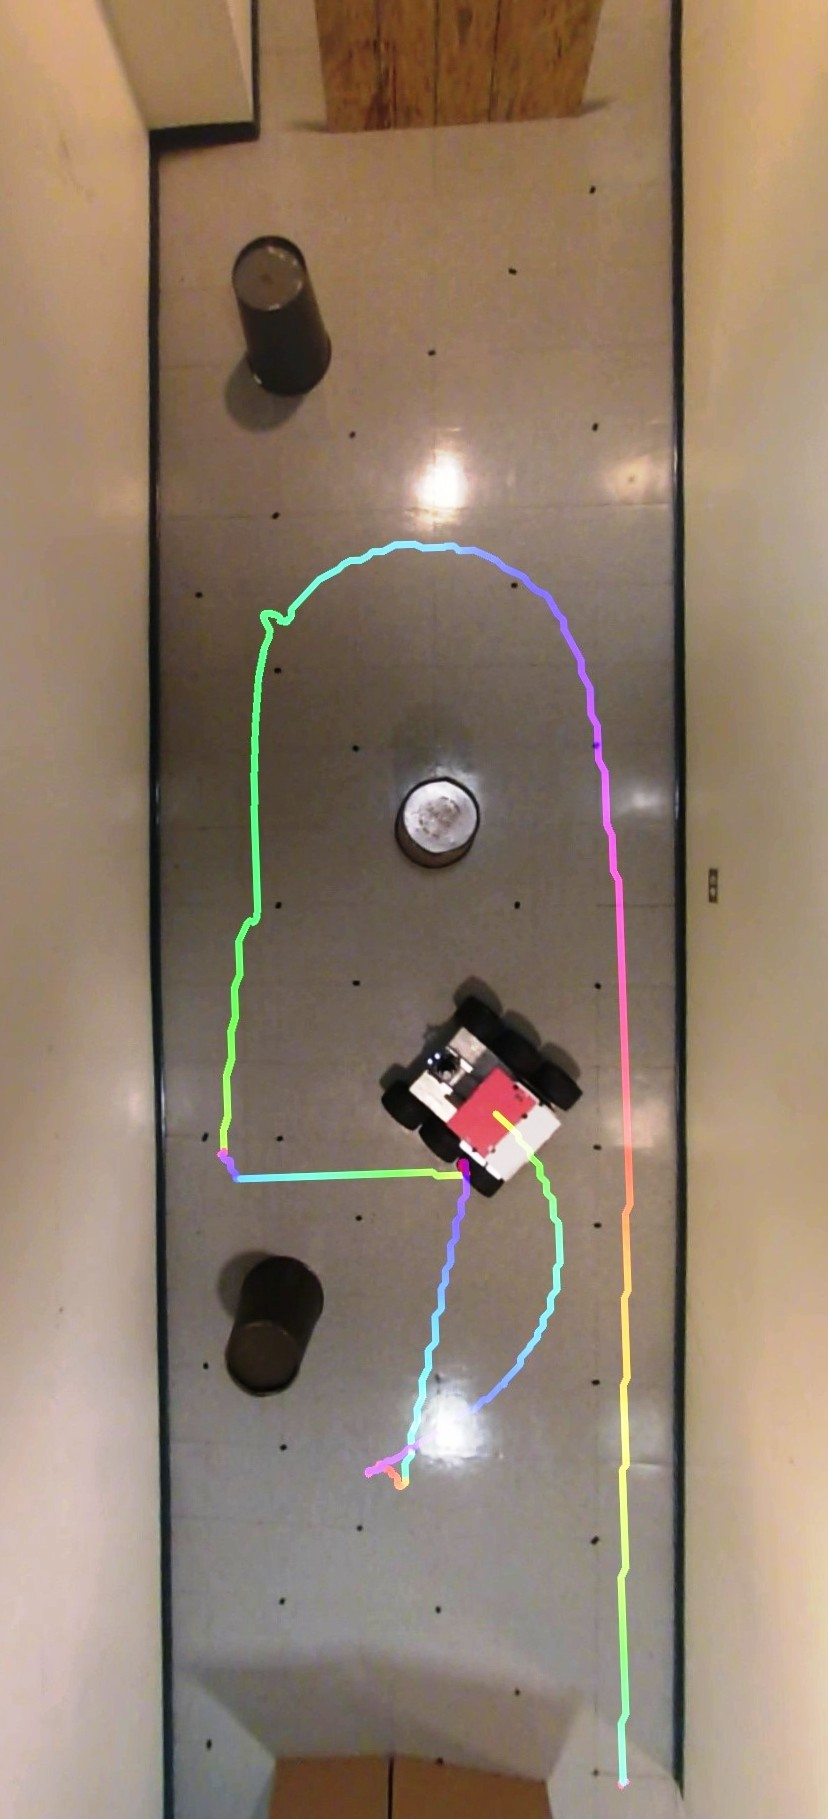
\includegraphics[height = 0.9\textheight]{overhead_path}
\caption{Controlled environment and path reconstructed by an overhead camera.}
\label{fig:overhead_path}
\end{figure}
To look at the effectiveness of the SLAM algorithm, some knowledge of the actual path taken by the robot is required for comparison. This is reconstructed using an overhead camera and the movement of the robot in the video is recorded. While this may not give the actual path or the ground truth accurately, it gives a reasonable estimate of it to within a few inches of deviation. A sample reconstructed path is shown in Figure~\ref{fig:overhead_path}. The camera based reconstructed path is also shown in all the plots of SLAM reconstructions for comparison. In the run, the robot starts at the bottom right corner and ends at the position shown.

Since the map is constructed relative to the starting location, the robot is always assumed to be starting at the origin in all the reconstructions.

\subsection{Using Point Features}
\label{sec: point_result}
In Figure~\ref{fig:overhead_path} the cylinders around which the robot travels are the point features that are to be detected. The algorithm used is the same as described in Section~\ref{sec: spikeAlgo}. Using just the jump in distance as a landmark results in a large number of spurious landmarks. As discussed in Section~\ref{sec: spikeAlgo}, it is therefore necessary to filter through the candidate landmarks using preexisting knowledge as previously described. The minimum number of points that need to be on the candidate landmark is chosen to be 11 for this particular arrangement. This is a tuning parameter which is decided after a few trials for optimized performance. The other tuning parameters include the thresholding for the range that the angular width can be in based on the radius of the cylinders which is $ 0.1524 $ m and the threshold for the curvature of the candidate landmark which is chosen to be $ 9 \% $. These tuning parameters are chosen only once for a particular environment. 

Once the feature extractor is tuned, the SLAM algorithm itself needs to be tuned based on the estimated noise factors for the various sensors. The SLAM algorithm is more robust to these parameters than the feature extractor and hence, a range of values yield good performance. Another part of the algorithm that needs to be tuned carefully is the landmark association. For point features in the map, the Euclidean distance between the detected and the preexisting cylinder is used. Hence, the maximum allowable distance for association needs to be set. That distance has to be large enough to accommodate for a particular landmark not being seen for a few steps and then being detected. It also should not be too large since this will result in wrong associations which will correct the path of the robot in a completely different way than the correct associations. Hence this parameter is also a function of the order of distances in the arena and is chosen to be $ 2 m $, in these experiments.
\begin{figure}
\centering
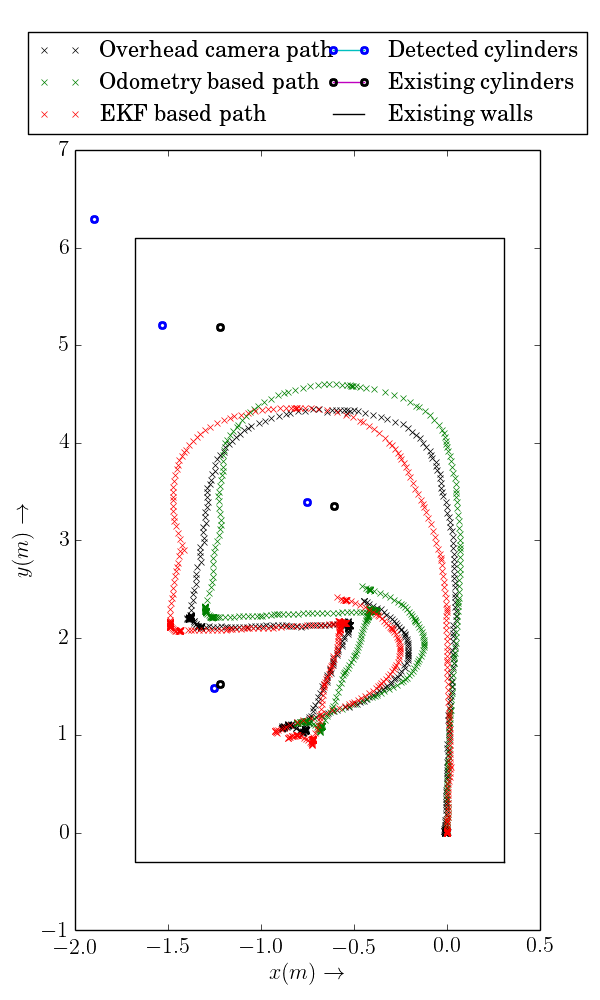
\includegraphics[height = 0.9\textheight]{cylinder}
\caption{Controlled environment and path reconstructed by detecting point features in LIDAR data. Path starts from the origin.}
\label{fig:cylinder_result}
\end{figure}

With these parameters, the path of the robot is reconstructed as seen in Figure~\ref{fig:cylinder_result}. We can see that it tries to correct the path towards the ground truth compared to the odometry based estimate, but it overcompensates frequently. This demonstrates the disadvantage of the conservative nature of the filters used. Since the focus is to not allow any spurious landmarks, the actual landmarks are also missed in a number of time steps. This effects the reconstruction mainly when there is only one landmark in the field of view of the LIDAR. 

In the part of the path that is shown in the upper right quadrant in Figure~\ref{fig:cylinder_result}, as soon as the robot has lost the first cylinder from its field of view, only the middle cylinder is seen for sometime until the robot turns and the third cylinder comes close enough to be resolved. This is the time interval when the SLAM reconstructed path deviates from the actual path as the heading was being previously corrected using the cylinders detected, but when the landmark is missed, the pure odometry keeps moving it in the same direction. A similar effect is seen in the upper right corner when the only cylinder that can be seen is the uppermost one. This compounds the error previously accumulated. It is only when the robot is able to see both the lower and the middle cylinders simultaneously, that the path is corrected. This overcompensation also results in a corresponding error in the reconstruction of the environment. This error as well as error in the end position of the robot is seen in Table~\ref{tab:cylinder_results}.

\begin{table}
\caption{Errors in environment reconstruction using point features.}
\label{tab:cylinder_results}
\begin{tabular}{| l | c | c | c |}
\hline ~ & Actual Position (x,y) & Detected Position (x,y) & Error(m)\\
\hline Cylinder 1 & (-1.2192,1.524) & (-1.2525,1.4851) & 0.002622 \\ 
\hline Cylinder 2 & (-0.6096,3.3528) & (-0.7522,3.3942) & 0.022048 \\ 
\hline Cylinder 3 & (-1.2192,5.1816) & (-1.5308,5.2055) & 0.097665 \\ 
\hline End Position & (-0.4459,2.3715) & (-0.5917,2.4141) & 0.023072 \\
\hline 
\end{tabular} 
\end{table}

\subsection{Using linear features}
\label{sec: hough_results}

In the controlled environment of Figure~\ref{fig:overhead_path}, the linear features are the 4 walls enclosing the space. For wall detection, two algorithms are discussed in Section~\ref{sec:extraction}. The RANSAC based algorithm, when implemented in the way discussed is seen to be not robust in Figure~\ref{fig: ransac_bad}. When used in SLAM it generates a number of spurious landmarks which result in wrong data association and subsequent correction. This results in the reconstruction being highly erroneous. 

Hence the Hough transform based algorithm is used. As described in Section~\ref{sec:hough}, the only tuning parameters for that algorithm are the pixel and angular resolution and threshold for line detection. Since these are broad parameters any reasonable value may be chosen. Since we use an image of 1000~$ \times $~1000 pixels to represent 10~m~$ \times $~10~m space in the real world, the physical significance of the pixel resolution is the minimum distance in centimeters that walls need to be far from each other for them to be considered as 2 individual walls instead of one. The angular resolution is useful as it avoids finding multiple walls with small angles between them. This is especially useful while reconstructing indoor environments as most walls tend to intersect at right angles hence corresponding to a very low probability that the actual line features intersect at a small angle. In this arena, an angular resolution of $ 10^\circ $ and a distance resolution of 2~cm is chosen. This allows a good reconstruction while speeding up the Hough transform itself as the size of the accumulator from equation \ref{eq:hough3} is reduced. 

\begin{figure}
\centering
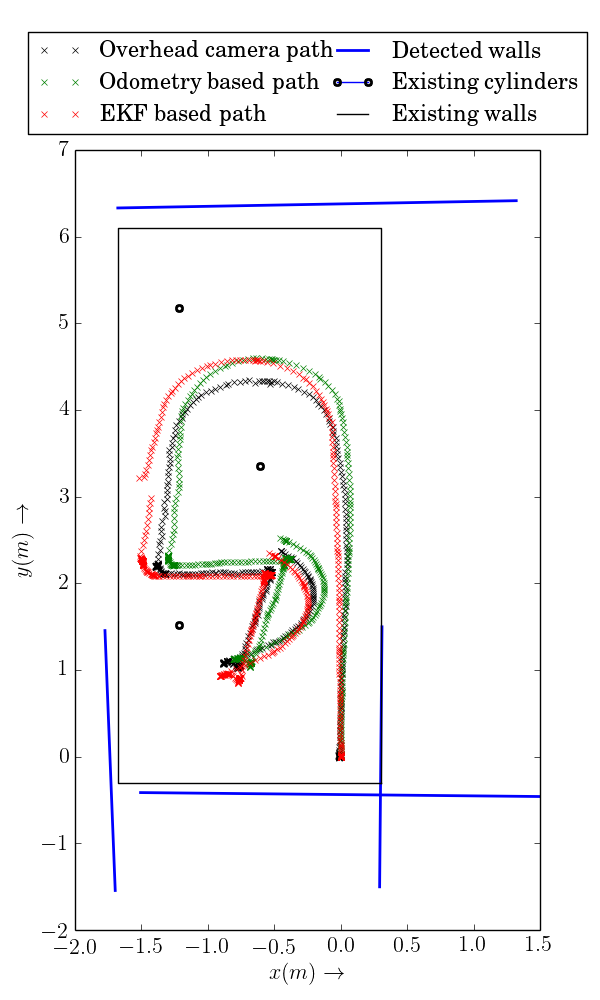
\includegraphics[height = 0.9\textheight]{walls}
\caption{Controlled environment and path reconstructed by detecting linear features in LIDAR data. Path starts from the origin.}
\label{fig:wall_result}
\end{figure}

The noise covariances for the encoder and LIDAR are kept the same as in Section~\ref{sec:Spike_results} since the same instruments are used. The only part that needs to be different from Section~\ref{sec: point_result} is the data association. There are a large number of ways that a linear feature can be associated. The simplest method is the Euclidean distance. This is feasible as the lines are represented in the normal form as shown in Figure~\ref{fig: normal_form}. Hence, the coordinates of the line are actually the point of intersection of the normal from the origin. If there is a difference in either angle or distance, the point of intersection will move. Hence the Euclidean distance between the detected and preexisting lines gives a good measure for association.

However, using solely the Euclidean distance is seen to have a drawback. It can lead to a wrong association when the lines are sufficiently close to the origin, such as in the bottom right corner of Figure~\ref{fig:overhead_path}. Then, the Euclidean distance between the points of intersection of the normals is lower than the threshold causing the 2 perpendicular walls to be associated as the same wall. Hence, it is necessary to add another heuristic to avoid this. The heuristic added in this implementation was based on the angle of intersection between the walls. The additional condition is that, even if Euclidean distance is small, if the angle of intersection is not close to 0 or 180 degrees, then the features are not associated with each other. With this addition, the path of the robot was reconstructed as shown in Figure~\ref{fig:wall_result}.


It is seen that the SLAM reconstruction is able to track the actual position for the most part except during the turn at the top and in a part close to the left wall. In the former case, the deviation from the path is mainly due to the odometry. This occurs as the robot has turned sufficiently to lose sight of the right wall and there are only small sections of the back and left wall in its field of view. This causes the walls to be not detected and emphasis is therefore, given to the odometry. In the part close to the left wall, the robot is moving slightly towards the wall in the ground truth whereas according to the odometry it is almost parallel. Since the only wall that the LIDAR can see at this point is the left wall and since the left wall has only recently been observed there is a greater tendency to move the estimated wall than the robot. This is also the reason in Figure~\ref{fig:wall_result}, for the left wall to be seen at an angle. Once the robot close enough to see the back wall, the SLAM reconstruction does a large correction resulting in the jump seen. The errors in the environment reconstruction as well as the path are shown in Table~\ref{tab:wall_results}. 

\begin{table}
\caption{Errors in environment reconstruction using linear features.}
\label{tab:wall_results}
\begin{tabular}{| l | c | c | c |}
\hline ~ & Actual Position (x,y) & Detected Position (x,y) & Error(m)\\
\hline Wall 1 & (0,-0.3048) & (-0.0066 -0.4371) & 0.017547 \\ 
\hline Wall 2 & (0.3048,0) & (0.3018,-0.0018) & 0.000012 \\ 
\hline Wall 3 & (0,6.096) & (-0.1784,6.3731) & 0.108611 \\ 
\hline Wall 4 & (-1.6764,0) & (-1.7358,-0.0447) & 0.005526 \\
\hline End Position & (-0.4459,2.3715) & (-0.5362,2.3477) & 0.008721 \\
\hline 
\end{tabular} 
\end{table}

\subsection{Using a combination of point and linear features}
\label{sec:combo_result}

As seen in Section~\ref{sec:slam_process}, the implementation of SLAM algorithm is designed to use both kinds of features simultaneously. With all the implementation details as in Sections \ref{sec:Spike_results} and \ref{sec: hough_results}, the reconstructed path is shown in Figure~\ref{fig:combo_result}.

\begin{figure}
\centering
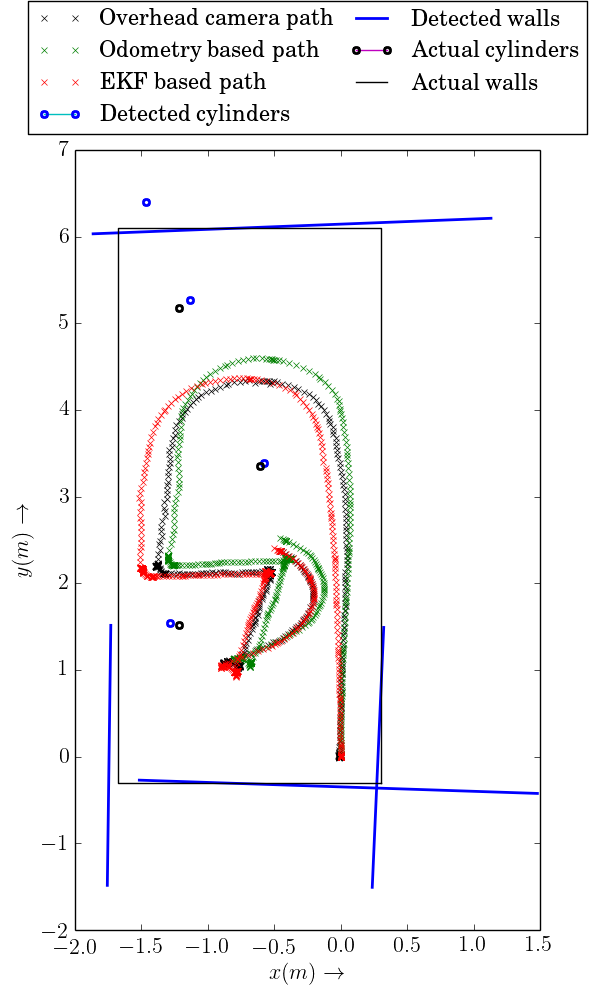
\includegraphics[height = 0.9\textheight]{both}
\caption{Controlled environment and path reconstructed by detecting both point and linear features in LIDAR data. Path starts from the origin}
\label{fig:combo_result}
\end{figure}


From the path, it is seen that a few of the errors from the previous two reconstructions have been corrected. For example, in Figure~\ref{fig:cylinder_result}, there is a large error in the top left part of the plot due to the cylinder not being detected robustly. In this path, the lack of the  cylinder feature is compensated for by using the walls. Since it is a corner region the algorithm is able to correct both position and orientation. In Figure~\ref{fig:wall_result}, there is a jump in the path near the left wall, and the left wall is reconstructed at an angle, as discussed in Section~\ref{sec: hough_results}. When the robot is traveling parallel to the left wall, it has 2 cylinders in its field of view, and hence, this jump is avoided.

There are still deviations from the path near the left wall as both the linear features based and the point features based reconstructions had both deviated at that region, a combination of the two cannot yield an accurate reconstruction, though it can be better than either one individually. The environment reconstruction errors are tabulated in Table~\ref{tab:combo_results}

\begin{table}
\caption{Error in environment reconstruction using combination of linear and point features}
\label{tab:combo_results}
\begin{tabular}{| l | c | c | c |}
\hline ~ & Actual Position (x,y) & Detected Position (x,y) & Error(m)\\
\hline Cylinder 1 & (-1.2192,1.524) & (-1.2856,1.5376) & 0.004602 \\ 
\hline Cylinder 2 & (-0.6096,3.3528) & (-0.5768,3.3911) & 0.002543 \\ 
\hline Cylinder 3 & (-1.2192,5.1816) & (-1.1308,5.2717) & 0.015932 \\
\hline Wall 1 & (0,-0.3048) & (-0.0177,-0.3476) & 0.002145 \\ 
\hline Wall 2 & (0.3048,0) & (0.2805,-0.0080) & 0.000654 \\ 
\hline Wall 3 & (0,6.096) & (-0.3663,6.1225) & 0.134878 \\ 
\hline Wall 4 & (-1.6764,0) & (-1.7436,0.0152) & 0.004747 \\
\hline End Position & (-0.4459,2.3715) & (-0.5013,2.4103) & 0.00457 \\
\hline 
\end{tabular} 
\end{table}

To compare the reconstructions, we can compare the landmark error values from the tables. In Table~\ref{tab:combo_results}, the total of all the cylinder errors is 0.0231 m. The corresponding errors in Table~\ref{tab:cylinder_results} add up to 0.1223 m. Hence, in terms of finding the location of the cylinders using the combination of both kinds of features reduces the error by 81.1\%. Similarly The total error in walls, for the combination of both is 0.142 and with just linear features is 0.132. Hence, using the combination of features is seen to increase the error, but only by 8\%. If we consider the end position of the robot, we see that compared to the point features based reconstruction, there is a 80\% reduction of error in the reconstruction using both types of features and a 47.5\% reduction compared to using only linear features. 

\subsection{Uncontrolled environment with linear features}

\begin{figure}
    \centering
    \begin{subfigure}[b]{0.45\textwidth}
	    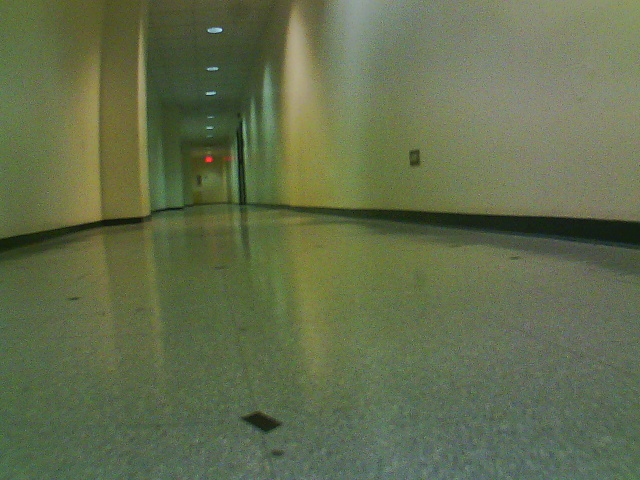
\includegraphics[width=\textwidth]{corr1}
    \end{subfigure}
    \quad %add desired spacing between images, e. g. ~, \quad, \qquad, \hfill etc.
      %(or a blank line to force the subfigure onto a new line)
    \begin{subfigure}[b]{0.45\textwidth}
        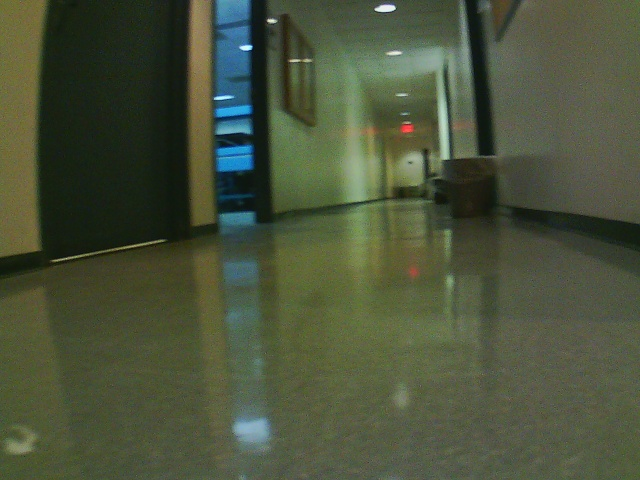
\includegraphics[width=\textwidth]{corr2}
    \end{subfigure}%

    \caption{Passages forming an uncontrolled environment}
    \label{fig:onboard_1}
\end{figure}

\begin{figure}
    \centering
    \begin{subfigure}[b]{0.45\textwidth}
	    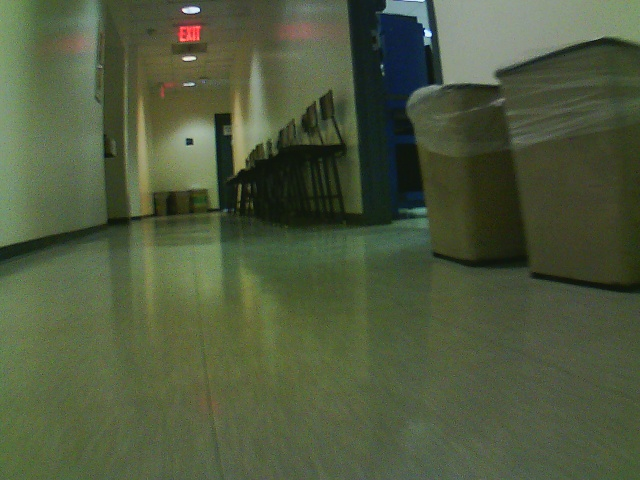
\includegraphics[width=\textwidth]{corr3}
    \end{subfigure}
    \quad %add desired spacing between images, e. g. ~, \quad, \qquad, \hfill etc.
      %(or a blank line to force the subfigure onto a new line)
    \begin{subfigure}[b]{0.45\textwidth}
        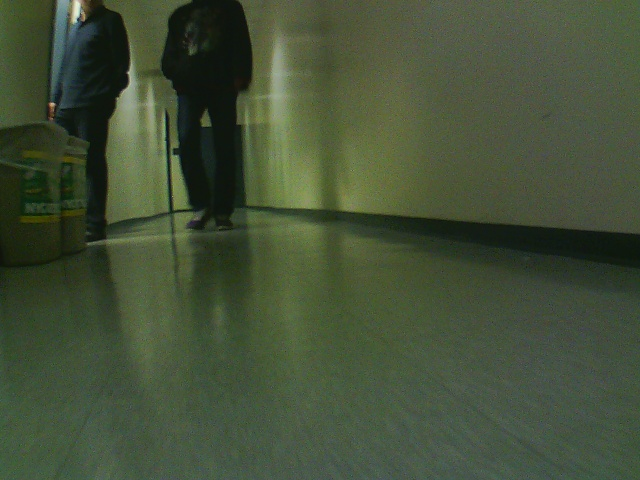
\includegraphics[width=\textwidth]{corr_human}
    \end{subfigure}%

    \caption{Obstacles in an uncontrolled environment}
    \label{fig:onboard_2}
\end{figure}
The primary purpose of implementing EKF SLAM is to run it in real time. For this, it is essential that the tuning parameters previously discussed should not need to be tuned for each specific arena configuration. Hence, a longer run in an uncontrolled environment  with the same tuning parameters is analyzed.

From Section~\ref{sec:combo_result}, it is clear that the linear features based SLAM is relatively accurate compared to point features based SLAM. Although the combination of both walls and cylinders for SLAM gave the best results, the feature extractor for cylinder is seen to be conservative and not entirely robust. In Section~\ref{sec:hough} it was shown that the Hough transform based linear feature extractor is robust to humans in its field of view. Hence for a long range uncontrolled indoor environment, the linear feature based SLAM is an ideal candidate. 

To test this, the robot is driven around a long passage which has both open and closed doors on either side as seen in Figure~\ref{fig:onboard_1} There are also people walking around and entering and leaving through those doors. As seen in Figure~\ref{fig:onboard_2}, there are also other unintentional point features in the environment. 

This gives a challenge for both EKF based SLAM and for the Hough feature extractor. The correction should ideally be made based only on walls and not other lines such as door ways etc. For SLAM itself, since the distance traveled is much larger and the velocity with which the robot moves is also larger, the encoders drift by a considerable amount as seen in Figure~\ref{fig:big_run}. Since the run is in a larger environment, the ground truth is approximated manually, without any overhead camera data. It can be seen that linear feature based SLAM does a good job in estimating the path traveled compared to the odometry. It does not completely reconstruct the ground truth due to the large number of disturbances throughout it's path such as doors. Towards the end of the run, a number of estimated wall are seen due to the shape of the passages in that region. 

\begin{figure}
\centering
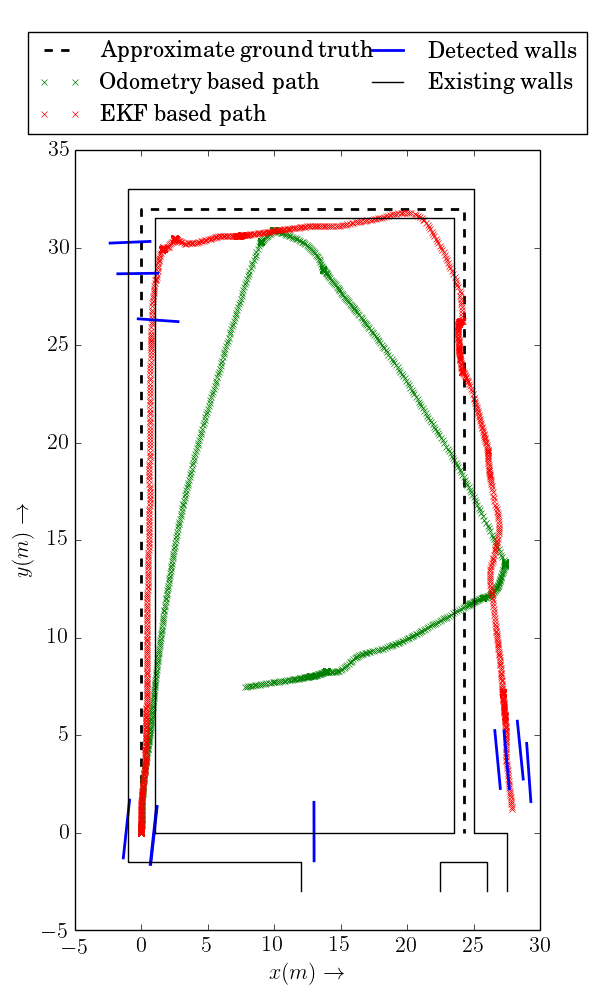
\includegraphics[height = 0.9\textheight]{big_run}
\caption{Uncontrolled environment and path reconstructed by detecting linear features in LIDAR data. Path starts from the origin.}
\label{fig:big_run}
\end{figure}

Hence, it is seen that in an uncontrolled environment, the Hough transform based linear feature detector performs well at reconstructing the path of the robot, even though the reconstruction of the environment is not accurate. It is also seen that the tuning parameters chosen in Section~\ref{sec:Spike_results} and \ref{sec: hough_results}, are robust and do not need to be changed for similar environments.  
\chapter{Conclusion}

\bibliographystyle{IEEEtran}
\bibliography{IEEEabrv,bibliography}

%\include{bib}
\end{document}